% =====================================================================
%  Final-Year Research Project Report (CSC406S6 / CSC406M6)
%  A Deep Reinforcement Learning Approach for Proactive Load-Balancing
%  Controller Management in Software-Defined Networks
%
%  Overleaf: upload the whole "latex" folder (or the provided zip),
%  set the main document to main.tex and the compiler to pdfLaTeX.
%  Build locally:  pdflatex main && bibtex main && pdflatex main && pdflatex main
% =====================================================================
\documentclass[12pt,a4paper,oneside]{report}

% ---------- encoding, fonts, layout
\usepackage[T1]{fontenc}
\usepackage[utf8]{inputenc}
\usepackage{mathptmx}            % Times-compatible text and maths
\usepackage[scaled=0.92]{helvet}
\usepackage{microtype}
\usepackage[a4paper,left=1.25in,right=1in,top=1in,bottom=1in]{geometry}
\usepackage{setspace}
\onehalfspacing

% ---------- maths, tables, figures
\usepackage{amsmath,amssymb,bm}
\usepackage{graphicx}
\usepackage{booktabs,tabularx,multirow,longtable,array,makecell}
\usepackage{threeparttable}
\usepackage{float}
\usepackage[font=small,labelfont=bf,skip=6pt]{caption}
\usepackage{subcaption}
\usepackage{pdflscape}
\usepackage{xcolor}
\usepackage{enumitem}
\usepackage{listings}
\usepackage{fancyhdr}
\usepackage{titlesec}
\usepackage[nottoc]{tocbibind}
\usepackage{url}
\usepackage[hidelinks,bookmarksnumbered]{hyperref}
\urlstyle{tt}
\makeatletter\g@addto@macro{\UrlBreaks}{\do\_\do\/\do\.\do\-}\makeatother
\newcommand{\fitwidth}[1]{\resizebox{\ifdim\width>\linewidth\linewidth\else\width\fi}{!}{#1}}

\graphicspath{{figures/}}
\setlist{itemsep=2pt,topsep=4pt}
\renewcommand{\arraystretch}{1.15}
\setlength{\emergencystretch}{3em}
\newcolumntype{L}{>{\raggedright\arraybackslash}X}
\newcolumntype{P}[1]{>{\raggedright\arraybackslash}p{#1}}
\newcolumntype{C}{>{\centering\arraybackslash}X}

% ---------- algorithm float (no external algorithm package needed)
\newfloat{algorithm}{tbp}{loa}[chapter]
\floatname{algorithm}{Algorithm}
\floatstyle{ruled}
\restylefloat{algorithm}

% ---------- code listings
\definecolor{codebg}{HTML}{F6F6F4}
\lstset{basicstyle=\ttfamily\footnotesize, backgroundcolor=\color{codebg},
        frame=single, rulecolor=\color{gray!40}, breaklines=true,
        columns=fullflexible, keepspaces=true, xleftmargin=4pt, xrightmargin=4pt}

% ---------- headings and page style
\titleformat{\chapter}[display]{\normalfont\bfseries\Large}{\chaptertitlename\ \thechapter}{8pt}{\LARGE}
\titlespacing*{\chapter}{0pt}{0pt}{18pt}
\setlength{\headheight}{15pt}
\pagestyle{fancy}
\fancyhf{}
\fancyhead[L]{\small\nouppercase{\leftmark}}
\fancyfoot[C]{\thepage}
\renewcommand{\headrulewidth}{0.4pt}
\fancypagestyle{plain}{\fancyhf{}\fancyfoot[C]{\thepage}\renewcommand{\headrulewidth}{0pt}}

% ---------- shorthand
\newcommand{\rdqn}{RDQN}
\newcommand{\grurdqn}{GRU-RDQN}
\newcommand{\pmsd}[2]{$#1 \pm #2$}

% ---------- report metadata (edit here)
\newcommand{\reporttitle}{A Deep Reinforcement Learning Approach for Proactive Load-Balancing Controller Management in Software-Defined Networks}
\newcommand{\studentname}{M. Logadharsan}
\newcommand{\regno}{2021/SP/098}
\newcommand{\supervisor}{Dr. K. Thabotharan}
\newcommand{\department}{Department of Computer Science}
\newcommand{\faculty}{Faculty of Science}
\newcommand{\university}{University of Jaffna}
\newcommand{\coursecode}{CSC406S6 / CSC406M6 -- Research Project}
\newcommand{\submissiondate}{December 2026}

\begin{document}

% =====================================================================
%  FRONT MATTER
% =====================================================================
\pagenumbering{roman}
% ---------------------------------------------------------------- title page
\begin{titlepage}
  \centering
  \vspace*{0.4cm}
  {\large\textsc{\university}\par}
  \vspace{2pt}
  {\normalsize \faculty\ \textbullet\ \department\par}
  \vspace{1.6cm}
  {\LARGE\bfseries \reporttitle\par}
  \vspace{1.4cm}
  {\large Final-Year Research Project Report\par}
  \vspace{4pt}
  {\normalsize \coursecode\par}
  \vfill
  \begin{tabular}{rl}
    \textbf{Student:} & \studentname \\
    \textbf{Registration number:} & \regno \\[4pt]
    \textbf{Supervisor:} & \supervisor \\
  \end{tabular}
  \vfill
  {\normalsize A report submitted in partial fulfilment of the requirements of the\\
  Bachelor of Science (Honours) degree in Computer Science\par}
  \vspace{1cm}
  {\large \submissiondate\par}
\end{titlepage}

% ---------------------------------------------------------------- declaration
\chapter*{Declaration}
\addcontentsline{toc}{chapter}{Declaration}
I hereby declare that this research project report, entitled \emph{``\reporttitle''}, is my own work and has not been submitted, in whole or in part, for any other degree or qualification. Work by other authors is acknowledged in the text and listed in the references. The implementation, experiments and results reported here were carried out by me under the supervision of \supervisor.

\vspace{2cm}
\noindent
\begin{tabular}{@{}p{0.45\textwidth}p{0.45\textwidth}@{}}
\rule{5.5cm}{0.4pt} & \rule{5.5cm}{0.4pt}\\
\studentname\ (\regno) & Date\\[1.6cm]
\end{tabular}

\noindent I certify that the above statement is correct to the best of my knowledge, and that the report is suitable for submission.

\vspace{2cm}
\noindent
\begin{tabular}{@{}p{0.45\textwidth}p{0.45\textwidth}@{}}
\rule{5.5cm}{0.4pt} & \rule{5.5cm}{0.4pt}\\
\supervisor\ (Supervisor) & Date\\
\end{tabular}

% ---------------------------------------------------------------- acknowledgements
\chapter*{Acknowledgements}
\addcontentsline{toc}{chapter}{Acknowledgements}
I am grateful to my supervisor, \supervisor, for guidance and constructive feedback throughout this project. I thank the academic and technical staff of the \department, \university, for their support and for the facilities provided. I also acknowledge the creators of the Internet Topology Zoo and of the Abilene traffic-matrix archive, whose publicly available data made this study possible. Finally, I thank my family and friends for their encouragement.

% ---------------------------------------------------------------- abstract
\chapter*{Abstract}
\addcontentsline{toc}{chapter}{Abstract}
Distributed software-defined networks (SDN) use several controllers, but time-varying traffic can overload some controllers while others sit idle and still consume energy. Static controller placement and purely reactive switch migration address only part of this problem. This project investigates whether a deep reinforcement learning agent can manage controllers proactively at runtime. A Rainbow Deep Q-Network (RDQN), acting as a master controller, selects at each decision interval one of four action types: migrate a switch away from an overloaded controller, evoke a parked controller, park an underloaded controller, or take no action. A valid-action mask with feasibility checks keeps every chosen action executable, and a bounded reward combines switch--controller latency, modelled controller energy and traffic load balance. An optional gated recurrent unit (GRU) forecaster adds predicted loads to the state so that capacity can be added before overload occurs.

The framework was evaluated on five Internet Topology Zoo networks (9--197 switches) with chronologically split synthetic traffic, and on Abilene-derived traffic mapped to OS3E. Each learned policy was compared with threshold, random-valid and no-action baselines under identical conditions, and each test split was evaluated once after model selection. On held-out synthetic traffic, the selected learned policy achieved the highest reward on all five topologies and used 4.2--19.6\% less simulated energy than the threshold policy, with slightly higher average latency on four topologies. Forecasting helped on OS3E, improving reward from $-478.46$ to $-452.94$ and lowering energy from 442.18\,W to 380.89\,W relative to current-state RDQN, but did not help on Gridnet or BellCanada. In the real-traffic study, predictive GRU-RDQN had the better mean reward over three seeds ($-111.19\pm17.53$ versus $-121.80\pm20.14$), yet current-state RDQN won in two of the three seeds. Finally, the unchanged OS3E policies were run on a Mininet emulation with Open vSwitch and five separate os-ken OpenFlow controllers, replaying the same traces over three 150-step windows. All 687 controller start, stop and switch-handover operations succeeded, and GRU-RDQN made exactly the same decisions as in the simulator in every window, achieved the best reward in all three predictive-mode runs, and was unaffected by small measurement noise; a switch handover took 40\,ms and a controller start 0.65\,s on average. The contributions are a runtime migrate/park/evoke formulation, a leakage-controlled evaluation protocol, evidence that the value of forecasting is scenario-dependent, and an emulation backend that executes the learned decisions on a real OpenFlow data plane.


\vspace{6pt}
\noindent\textbf{Keywords:} software-defined networking; controller management; switch migration; energy efficiency; deep reinforcement learning; Rainbow DQN; GRU traffic forecasting.


\tableofcontents
\listoffigures
\listoftables
\listof{algorithm}{List of Algorithms}
\chapter*{List of Abbreviations}
\addcontentsline{toc}{chapter}{List of Abbreviations}
\begin{tabular}{@{}p{0.2\textwidth}p{0.72\textwidth}@{}}
C51 & Categorical distributional RL with 51 return atoms \\
CPP & Controller Placement Problem \\
DQN & Deep Q-Network \\
DRL & Deep Reinforcement Learning \\
GML & Graph Modelling Language \\
GRU & Gated Recurrent Unit \\
GRU-RDQN & Rainbow DQN whose state is augmented with GRU traffic forecasts \\
LSTM & Long Short-Term Memory \\
MAE & Mean Absolute Error \\
MDP & Markov Decision Process \\
MEC & Multi-access Edge Computing \\
MLP & Multi-Layer Perceptron \\
OD & Origin--Destination (traffic matrix) \\
OS3E & Internet2 Open Science, Scholarship and Services Exchange topology \\
OVS & Open vSwitch \\
PER & Prioritised Experience Replay \\
RDQN & Rainbow Deep Q-Network \\
RL & Reinforcement Learning \\
RMSE & Root Mean Squared Error \\
RTT & Round-Trip Time \\
SDN & Software-Defined Networking \\
UDP & User Datagram Protocol \\
\end{tabular}


% =====================================================================
%  MAIN MATTER
% =====================================================================
\clearpage
\pagenumbering{arabic}
\chapter{Introduction}
\label{ch:intro}

\section{Background and Motivation}
\label{sec:background}

Software-Defined Networking (SDN) separates the control plane from the data plane. Forwarding devices (switches) apply flow rules, while a logically centralised controller computes those rules and exposes the network to software through open interfaces such as OpenFlow~\cite{mckeown2008openflow,kreutz2015sdn}. Centralisation simplifies management, but a single physical controller limits scalability and is a single point of failure. Production deployments therefore use a \emph{distributed} control plane in which several controllers share the switches, with each switch assigned to one controller at a time.

A distributed control plane raises a second, operational question: \emph{which controllers should be active, and which switches should each one manage, as traffic changes?} The classical answer is the controller placement problem (CPP)~\cite{heller2012cpp,das2020survey}, which chooses controller locations and switch assignments at design time to minimise propagation delay, balance load or improve resilience. A placement that is good for average demand can become poor at runtime. Diurnal cycles, bursts and local hotspots can push one controller above its processing capacity while others remain lightly loaded. Overloaded controllers delay flow set-up, and controllers that remain active during low demand consume energy without doing useful work.

Two runtime mechanisms address these effects. \emph{Switch migration} reassigns a switch from an overloaded controller to a less loaded one~\cite{dixit2013elasticon,yeo2021sarlb}. \emph{Controller activation management} parks (deactivates) underused controllers to save energy and evokes (reactivates) them when demand rises. Each mechanism has trade-offs. Migration improves balance but can move a switch away from its nearest controller and increase latency. Parking saves energy but removes spare capacity. Evoking restores capacity at an energy cost. Choosing among these options at every interval is a sequential, multi-objective decision problem: an action taken now changes the controller state that later decisions start from.

Fixed threshold rules are simple and interpretable, but they react only after a threshold has been crossed and cannot weigh delayed consequences. Deep reinforcement learning (DRL) learns a policy from repeated interaction and optimises cumulative, not immediate, reward. It has therefore been applied to controller placement~\cite{bouzidi2022ddcp,chen2025mooo,farahi2026apdqn} and switch migration~\cite{yeo2021sarlb}. Most of this work, however, studies one mechanism in isolation. Placement methods decide where controllers should be. Migration methods move switches among an already fixed set of active controllers. Few studies let one learned policy decide jointly whether to migrate, park, evoke or wait. Fewer still examine whether a short-term \emph{traffic forecast} helps that policy act \emph{before} overload occurs.

This project is motivated by three observations. First, controller management is a runtime problem and should be evaluated on temporally ordered traffic, not on independent snapshots. Second, a reactive policy can only respond to overload once it has happened, whereas a forecast of near-future load could allow capacity to be prepared in advance. Third, a credible DRL evaluation needs chronologically separated training, validation and test data, baselines evaluated under identical conditions, and honest reporting of variance across training seeds~\cite{henderson2018matters,agarwal2021precipice}.

\section{Research Aim and Objectives}
\label{sec:objectives}

\paragraph{Aim.} To design, implement and evaluate a Rainbow-DQN-based framework for proactive runtime controller management in distributed SDN that jointly decides switch migration, controller parking, controller evoking and no action under dynamic traffic, balancing latency, energy and controller load.

\paragraph{Objectives.}
\begin{enumerate}[label=\textbf{O\arabic*.}, leftmargin=*]
  \item \textbf{Environment.} Develop an SDN controller-management environment built on real network topologies and temporal switch-level traffic. In this environment a learning agent can migrate switches, park underloaded controllers, evoke parked controllers or take no action, with action validity enforced and latency, energy and load balance measured.
  \item \textbf{Learning and fair evaluation.} Train topology-specific Rainbow DQN agents on five Internet Topology Zoo networks of increasing size. Evaluate them against threshold, random-valid and no-action baselines on chronologically held-out traffic under an identical protocol.
  \item \textbf{Forecast-assisted proactivity.} Integrate a GRU traffic forecaster as an optional predictive observation mode. Determine whether forecasting improves controller management relative to current-state RDQN, on synthetic traffic and on an Abilene-derived real-traffic case study.
\end{enumerate}

\section{Scope}
\label{sec:scope}

The study is carried out in a simulator. Controller locations are fixed graph nodes chosen by degree and closeness centrality; the agent manages their runtime state (active or parked) and the switch-to-controller mapping, but does not move controllers. Latency is the graph-derived propagation delay along shortest paths, and energy is a controller-state model (Section~\ref{sec:energy}), not a hardware measurement. The real-traffic case study maps measured Abilene traffic dynamics onto the OS3E topology; it is not measured OS3E production traffic. Deployment on an OpenFlow testbed such as Mininet~\cite{lantz2010mininet} is outside the scope of this report and is discussed as future work.

\section{Report Organisation}

Chapter~\ref{ch:related} reviews and compares related work by methodological category and identifies the research gap. Chapter~\ref{ch:method} presents the system architecture, the Markov decision process, the reward, the Rainbow DQN agent and the GRU forecaster. Chapter~\ref{ch:setup} describes the datasets, implementation, experimental protocol and metrics. Chapter~\ref{ch:results} reports and discusses the results, including ablations and limitations. Chapter~\ref{ch:conclusion} concludes and outlines future work. The appendices contain the complete result tables, hyperparameters, verification tests and reproduction commands.

\chapter{Related Work}
\label{ch:related}

This chapter groups related studies by \emph{methodological category}, not paper by paper: design-time placement, runtime migration, learning-based placement and mapping, forecast-assisted decision-making, and safety- and scale-oriented DRL. It then sets out the deep reinforcement learning and sequence-modelling foundations the project builds on, compares the closest approaches in Table~\ref{tab:litcompare}, and states the research gap.

\section{Design-Time Controller Placement}
\label{sec:rw-cpp}

Heller \emph{et al.}~\cite{heller2012cpp} formulated the controller placement problem: given a topology, choose $k$ controller locations to minimise average or worst-case switch--controller propagation latency. Later work, surveyed by Das \emph{et al.}~\cite{das2020survey}, extended the objective to capacity limits, load balance, reliability, inter-controller synchronisation and cost, solved with integer programming, clustering and metaheuristics. Two properties of this line of work are relevant here. First, it shows that the topology itself, through propagation delay, determines a latency floor that no assignment can beat. This project therefore evaluates on several real topologies (Topology Zoo~\cite{knight2011zoo}) and reports both average and worst-case latency. Second, placement is normally solved \emph{offline}, for a representative or peak demand. The resulting assignment is static, so it neither adapts when load shifts during the day nor exploits low-demand periods to save energy.

\section{Runtime Load Balancing by Switch Migration}
\label{sec:rw-migration}

Runtime approaches take the controller locations as given and adapt the switch-to-controller mapping. ElastiCon~\cite{dixit2013elasticon} introduced a switch-migration protocol and an elastic controller pool that can grow or shrink with load. This establishes that both migration and controller activation are feasible operations in a distributed control plane. Most subsequent schemes, reviewed in the 2025 survey of Liu \emph{et al.}~\cite{liu2025survey}, trigger migration from static or dynamic load thresholds and select the switch and target controller with heuristics. The survey identifies dynamic traffic, migration overhead and real-time decision quality as open challenges, and classifies existing methods as passive (reacting to overload) or proactive (anticipating it).

Reinforcement learning has been used to replace hand-crafted migration rules. SAR-LB~\cite{yeo2021sarlb} trains an RL agent to choose the switch and destination controller from resource-utilisation information and reports better load distribution than its compared schemes. Learned migration avoids manually tuned selection rules, but the action space contains migration only: the number of active controllers is fixed, so the policy cannot trade energy against capacity.

\section{Learning-Based Placement and Mapping}
\label{sec:rw-drl-cpp}

A parallel body of work applies DRL to placement and switch--controller mapping. Bouzidi \emph{et al.}~\cite{bouzidi2022ddcp} use a Deep Q-Network heuristic (DDCP) that jointly determines the number of controllers, their locations and the switch clusters, and validate it on the ONOS controller. Farahi \emph{et al.}~\cite{farahi2026apdqn} propose AP-DQN, a recent DQN-based approach to SDN controller placement. The work closest to this project algorithmically is MOOO-RDQN by Chen \emph{et al.}~\cite{chen2025mooo}. It applies a Rainbow-style DQN, with double Q-learning, prioritised replay, dueling networks, multi-step returns, noisy networks and distributional learning, to multi-objective controller placement and switch mapping, and adds a traffic-monitoring component for overload detection. MOOO-RDQN shows that Rainbow's sample-efficiency improvements carry over to SDN control problems with large discrete action spaces. Its decision, however, is \emph{where to place controllers and how to map switches}, not \emph{when to park, evoke or migrate} during operation.

\section{Forecast-Assisted Decision-Making}
\label{sec:rw-forecast}

A forecast lets a controller act on expected rather than observed load. Li \emph{et al.}~\cite{li2024mec} combine a CNN-LSTM traffic predictor with DRL for controller placement and edge selection in SDN-based multi-access edge computing, and report lower delay and energy than their baselines. The study supports the broader idea that predicted load improves DRL decisions. Its setting, though, is MEC task placement and edge selection, not runtime activation of SDN controllers, and it does not isolate the forecast's contribution by comparing the same agent with and without prediction. Recurrent networks are the usual forecasting tool for such traffic series. The gated recurrent unit (GRU)~\cite{cho2014gru} matches the long short-term memory network (LSTM)~\cite{hochreiter1997lstm} on many sequence tasks with fewer parameters~\cite{chung2014gru}, which makes it a reasonable lightweight forecaster for per-switch load.

\section{Safety and Scalability of DRL Load Balancing}
\label{sec:rw-safety}

Two recent directions address weaknesses of DRL controllers. Dinh \emph{et al.}~\cite{dinh2025safe} add a control-barrier-function layer to a DRL load balancer, so that actions taken during exploration and deployment satisfy safety constraints. Jha \emph{et al.}~\cite{jha2026federated} use asynchronous federated reinforcement learning across hierarchical controllers to scale load balancing to multi-domain networks. Both indicate where a single-agent simulator such as the one in this project is limited. Here, safety is enforced by an action mask and feasibility checks, which is weaker than a formal guarantee, and a separate agent is trained for each topology.

\section{Deep Reinforcement Learning Foundations}
\label{sec:rw-drl}

Deep Q-Networks~\cite{mnih2015dqn} approximate the action-value function with a neural network trained from a replay memory against a periodically updated target network. Rainbow~\cite{hessel2018rainbow} combines six extensions: double Q-learning, which reduces over-estimation~\cite{vanhasselt2016double}; prioritised experience replay~\cite{schaul2016per}; the dueling value/advantage architecture~\cite{wang2016dueling}; multi-step returns~\cite{sutton2018rl}; noisy linear layers for exploration~\cite{fortunato2018noisy}; and categorical distributional RL (C51)~\cite{bellemare2017c51}. Together these outperform each component alone. Large discrete action spaces in which many actions are illegal in a given state are commonly handled by \emph{invalid-action masking}~\cite{huang2022masking}, which this project adopts. Finally, DRL results are sensitive to random seeds and evaluation choices~\cite{henderson2018matters,agarwal2021precipice}. This motivates the multi-seed replication and the explicit uncertainty reporting used in Chapter~\ref{ch:results}.

\section{Comparative Synthesis and Research Gap}
\label{sec:gap}

\begin{table}[htbp]
\centering
\caption{Methodological comparison of the closest related approaches with this work.}
\label{tab:litcompare}
\small
\begin{tabularx}{\textwidth}{@{}P{2.55cm}P{2.25cm}P{1.85cm}LL@{}}
\toprule
\textbf{Work} & \textbf{Decision} & \textbf{Method} & \textbf{Proactivity / energy} & \textbf{Gap relative to this work} \\
\midrule
Heller \emph{et al.}~\cite{heller2012cpp}; Das \emph{et al.}~\cite{das2020survey} & Placement (offline) & Optimisa\-tion, heuristics & None; static design & No runtime adaptation \\
ElastiCon~\cite{dixit2013elasticon} & Migration, pool resizing & Protocol + heuristic & Reactive & Rule-based; no learning \\
SAR-LB~\cite{yeo2021sarlb} & Switch migration & RL & Reactive; no energy term & No park/evoke actions \\
DDCP~\cite{bouzidi2022ddcp}; AP-DQN~\cite{farahi2026apdqn} & Placement, clustering & DQN & Placement-level & Not runtime park/evoke/migrate \\
MOOO-RDQN~\cite{chen2025mooo} & Placement and mapping & Rainbow DQN & Monitoring for overload detection & Placement problem; no forecast ablation \\
Li \emph{et al.}~\cite{li2024mec} & Placement, edge selection (MEC) & DRL + CNN-LSTM & Forecast-assisted & MEC setting; no with/without-forecast comparison \\
Dinh \emph{et al.}~\cite{dinh2025safe} & Load balancing & DRL + barrier function & Safety layer & No controller activation \\
\textbf{This work} & \textbf{Migrate, park, evoke, no-op} & \textbf{Rainbow DQN, action mask} & \textbf{Optional GRU forecast; energy in reward} & Simulator; modelled energy; per-topology agents \\
\bottomrule
\end{tabularx}
\end{table}

Table~\ref{tab:litcompare} shows how these categories relate. Placement studies optimise an initial configuration. Migration studies rebalance a fixed set of active controllers. Learning-based placement brings DRL to the design-time decision. Forecast-assisted work shows that predicted load can guide decisions, but in neighbouring problems. Safety and federated studies harden DRL controllers but do not change what they decide. Across the literature, three points recur:

\begin{enumerate}[leftmargin=*]
  \item \textbf{Mechanisms are studied separately.} Migration (which mainly affects balance and latency) and controller activation (which mainly affects energy and capacity) are rarely chosen by the same learned policy, even though they act on the same controllers and interact.
  \item \textbf{The contribution of forecasting is rarely isolated.} Where forecasting is used, it is seldom compared against an otherwise identical current-state agent, so it is unclear when prediction actually helps.
  \item \textbf{Evaluation protocols are often weak.} Temporal leakage between training and test traffic, single-seed results and baselines evaluated under different conditions make reported gains hard to interpret.
\end{enumerate}

\paragraph{Research gap.} This project addresses a runtime controller-management framework in which \emph{one} learned discrete policy chooses among switch migration, controller parking, controller evoking and no action under temporally varying traffic, with explicit latency, energy and balance objectives. The policy is evaluated with chronological splits and identical baselines across topologies of different scale, and a matched current-state versus GRU-forecast comparison measures whether proactivity adds value. The aim is not to outperform placement methods on their own problem. Published percentage improvements from those studies use different problems, traffic and metrics, so they are compared methodologically (Section~\ref{sec:compare-existing}) rather than numerically.

\chapter{Methodology}
\label{ch:method}

This chapter describes the proposed approach: the system architecture, the formal model of the controller-management problem, the Markov decision process (MDP) solved by the agent, the reward, the Rainbow DQN learner, the GRU forecaster and its integration, and the baselines. Each section ends with the rationale for its main design choices.

\section{System Architecture and Workflow}
\label{sec:architecture}

Figure~\ref{fig:architecture} shows the architecture. It has four parts.
\begin{enumerate}[leftmargin=*]
  \item A \textbf{data layer} turns a Topology Zoo graph into a switch-to-controller delay matrix and supplies a normalised switch-load trace, split chronologically into training, validation and test segments.
  \item A \textbf{controller-management environment}, implemented with the Gymnasium interface~\cite{towers2024gymnasium}, holds the controller states and the switch mapping. It detects overload and underload, exposes the set of currently valid actions, applies the chosen action and returns the next state, a reward and performance metrics.
  \item A \textbf{Rainbow DQN agent}, logically located in the master controller, maps the state to an action.
  \item An optional \textbf{GRU forecaster} predicts near-future switch loads. In \emph{predictive mode} the forecasts are appended to the state and used to anticipate overload.
\end{enumerate}

The same environment code is reused unchanged by the Mininet emulation backend (Section~\ref{sec:mininet-setup}), where it is fed measured instead of trace loads and its decisions are carried out on emulated switches and controller processes.

At each decision interval $t$ the workflow is: (i) observe the state $s_t$; (ii) compute the valid action set $\mathcal{V}(s_t)$; (iii) select $a_t\in\mathcal{V}(s_t)$; (iv) execute $a_t$ and compute the reward $r_t$ from the resulting configuration; (v) advance the traffic trace by one row, recompute controller loads and, in predictive mode, refresh the forecast to produce $s_{t+1}$; and (vi) during training, store the transition and update the network.

\begin{figure}[htbp]
  \centering
  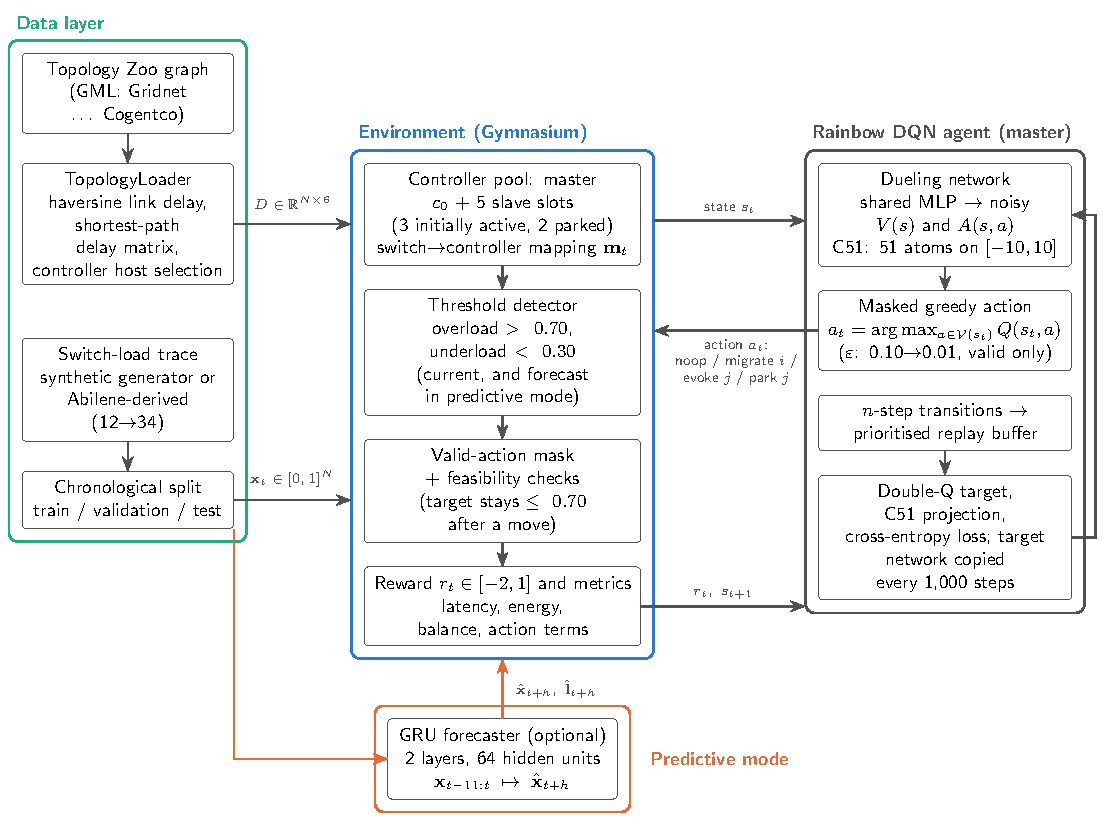
\includegraphics[width=\textwidth]{architecture}
  \caption{Architecture of the proactive controller-management framework. Orange elements are active only in predictive mode.}
  \label{fig:architecture}
\end{figure}

\section{System Model}
\label{sec:system-model}

\paragraph{Topology and controllers.} The network is an undirected graph $G=(\mathcal{S},\mathcal{E})$ with $N=|\mathcal{S}|$ switches. Each link $(u,v)$ has a propagation delay $d_{uv}=\max(\text{dist}_{\text{hav}}(u,v)/200,\ 0.1)$\,ms. Here $\text{dist}_{\text{hav}}$ is the great-circle distance in km between node coordinates, and 200\,km/ms approximates signal speed in fibre; links without coordinates receive 1\,ms. There are $K=6$ controller slots $\mathcal{C}=\{c_0,\dots,c_5\}$ hosted on the six nodes with the highest degree, with ties broken by closeness centrality. Slot $c_0$ is the master controller, which runs the agent and never manages switches. Slots $c_1$--$c_3$ start \emph{active} and $c_4$, $c_5$ start \emph{parked}. Let $D\in\mathbb{R}^{N\times K}$ be the shortest-path delay from each switch to each controller host.

\paragraph{Traffic and controller load.} At interval $t$ the trace supplies $\mathbf{x}_t\in[0,1]^N$, the normalised load of every switch. Let $A_t$ denote the set of active slave controllers and $m_t(i)\in A_t$ the controller of switch $i$. The load of an active controller is the \emph{mean} load of its switches:
\begin{equation}
  \ell_{j,t} = \frac{1}{|\{i:m_t(i)=j\}|}\sum_{i:\,m_t(i)=j} x_{i,t}, \qquad j\in A_t .
  \label{eq:load}
\end{equation}
A mean rather than a sum keeps $\ell_{j,t}$ in $[0,1]$ and comparable with fixed thresholds across topologies whose controllers serve very different numbers of switches. At reset, each switch is assigned to its nearest active controller according to $D$.

\paragraph{Energy model.}
\label{sec:energy}
The energy model follows controller state: the master consumes $E_m=50$\,W, each active slave $E_a=100$\,W and each parked slave $E_p=10$\,W, so $E_t=E_m+|A_t|E_a+|P_t|E_p$, where $P_t$ is the set of parked slaves. The initial configuration consumes 370\,W. This is a relative model used consistently for every policy; it is not a hardware measurement.

\section{Markov Decision Process Formulation}
\label{sec:mdp}

\paragraph{State.} In \emph{current mode} the observation is
\begin{equation}
  s_t = \big[\,\bm{\ell}_t,\ \mathbf{b}_t,\ \mathbf{m}_t\,\big]\in[0,1]^{2K+N},
\end{equation}
where $\bm{\ell}_t\in[0,1]^K$ are the controller loads (zero for parked slots), $\mathbf{b}_t\in\{0,1\}^K$ marks active controllers (the master is always 1), and $\mathbf{m}_t$ holds each switch's controller index divided by $K-1$. In \emph{predictive mode} the GRU forecast $\hat{\mathbf{x}}_{t+h}$ and the forecast controller loads $\hat{\bm{\ell}}_{t+h}$ (Eq.~\ref{eq:load} applied to $\hat{\mathbf{x}}_{t+h}$ under the current mapping) are appended:
\begin{equation}
  s^{\text{pred}}_t = \big[\,\bm{\ell}_t,\ \mathbf{b}_t,\ \mathbf{m}_t,\ \hat{\mathbf{x}}_{t+h},\ \hat{\bm{\ell}}_{t+h}\,\big]\in[0,1]^{2K+2N+K}.
\end{equation}
For OS3E ($N=34$) the state therefore has 46 elements in current mode and 86 in predictive mode.

\paragraph{Actions.} The discrete action space uses \emph{stable slots}, so an action index always means the same thing:
\begin{equation}
  \mathcal{A}=\{0\}\ \cup\ \{1,\dots,N\}\ \cup\ \{N{+}1,\dots,N{+}5\}\ \cup\ \{N{+}6,\dots,N{+}10\},
\end{equation}
namely no-op; migrate switch $i$; evoke slave $c_j$; park slave $c_j$. The size is $|\mathcal{A}|=N+11$, which is 20 actions for Gridnet and 208 for Cogentco. A migrate action names only the switch. The environment chooses the least-loaded feasible active target, which keeps the action space linear in $N$ instead of $N\times K$. Stable slots were introduced after an earlier implementation, in which park/evoke indices depended on the current controller state, was found to give the same index different meanings over time (Appendix~\ref{app:verification}).

\paragraph{Transitions and episodes.} The chosen action changes the mapping and the controller states. The trace then advances by exactly one row, so every step is one decision interval. Episodes last 1,000 steps during training and 500 steps during evaluation, and each episode starts at a specified index of the trace.

\section{Thresholds, Valid Actions and Feasibility}
\label{sec:valid}

An active controller is \emph{overloaded} if $\ell_{j,t}>\theta_{\text{over}}=0.70$ and \emph{underloaded} if $\ell_{j,t}<\theta_{\text{under}}=0.30$. Algorithm~\ref{alg:valid} computes the valid action set. No-op is always valid. Migration and evoking are offered only when some controller is overloaded. Parking is offered only for an underloaded controller whose switches can be absorbed by the remaining active controllers without overloading any of them. A migration is valid only if the chosen target stays at or below $\theta_{\text{over}}$ after the move. When a controller is evoked, the environment immediately moves the most heavily loaded switch of the most overloaded controller onto it, so that the new capacity is used at once.

In predictive mode, the overload set is the union of currently overloaded and \emph{forecast}-overloaded controllers, so migration and evoking can become available before overload occurs. Two conservative rules limit the influence of forecasts: a migration must also keep the target's \emph{forecast} load at or below $\theta_{\text{over}}$, and parking is based on \emph{current} underload only, so a forecast alone never removes capacity.

\begin{algorithm}[htbp]
\caption{Valid-action set $\mathcal{V}(s_t)$}
\label{alg:valid}
\small
\begin{tabbing}
\hspace{1.2em}\=\hspace{1.2em}\=\hspace{1.2em}\=\kill
\textbf{Input:} mapping $m$, active set $A$, parked set $P$, loads $\bm{\ell}$, forecast loads $\hat{\bm{\ell}}$ (predictive mode)\\
1:\> $\mathcal{V}\leftarrow\{0\}$ \hfill \emph{no-op is always valid}\\
2:\> $O\leftarrow\{j\in A:\ell_j>0.70\}$;\quad \textbf{if} predictive \textbf{then} $O\leftarrow O\cup\{j\in A:\hat\ell_j>0.70\}$\\
3:\> $U\leftarrow\{j\in A:\ell_j<0.30\}$ \hfill \emph{current underload only}\\
4:\> \textbf{if} $O\neq\emptyset$ \textbf{then}\\
5:\>\> \textbf{for each} switch $i$ with $m(i)\in O$ \textbf{do}\\
6:\>\>\> $k\leftarrow\arg\min_{j\in A\setminus\{m(i)\}}\ \ell_j$ \quad (predictive: $\max(\ell_j,\hat\ell_j)$)\\
7:\>\>\> \textbf{if} load of $k$ after moving $i$ $\le0.70$ (and forecast load $\le0.70$) \textbf{then} add \emph{migrate}$(i)$\\
8:\>\> add \emph{evoke}$(j)$ for every $j\in P$\\
9:\> \textbf{if} $|A|>1$ \textbf{then}\\
10:\>\> \textbf{for each} $j\in U$ \textbf{do}\\
11:\>\>\> tentatively reassign $j$'s switches, heaviest first, to the least-loaded remaining controller\\
12:\>\>\> \textbf{if} no remaining controller exceeds $0.70$ \textbf{then} add \emph{park}$(j)$\\
13:\> \textbf{return} $\mathcal{V}$
\end{tabbing}
\end{algorithm}

\paragraph{Rationale.} Masking invalid actions~\cite{huang2022masking} keeps the agent from spending experience on impossible actions and keeps it from ever executing an unsafe reassignment. It also means that all policies, learned and baseline, choose from exactly the same legal moves, which keeps the comparison fair. The fixed 0.30/0.70 thresholds were kept unchanged throughout the project so that later implementation fixes were not confounded with changes to the problem definition.

\section{Reward Design}
\label{sec:reward}

The step reward combines three normalised operating costs with action-dependent shaping terms, and is clipped to $[-2,1]$:
\begin{equation}
  r_t=\operatorname{clip}_{[-2,1]}\Big(-\big(0.35\,\tilde L_t+0.35\,\tilde E_t+0.30\,\tilde B_t\big)+\alpha_t-\omega_t\Big),
  \label{eq:reward}
\end{equation}
where
\begin{align}
  \tilde L_t &= \frac{\frac{1}{N}\sum_i D_{i,m_t(i)}}{\max D}, &
  \tilde E_t &= \frac{E_t-E_{\min}}{E_{\max}-E_{\min}}, &
  \tilde B_t &= \frac{\min(\mathrm{CV}(\bm{\ell}_{A_t}),\,2)}{2}.
\end{align}
$\tilde L_t$ is the average switch--controller delay normalised by the largest delay in the topology. $\tilde E_t$ normalises energy between $E_{\min}=190$\,W (one active slave) and $E_{\max}=550$\,W (all five active). $\tilde B_t$ is the coefficient of variation of active-controller loads, capped at 2.

The shaping term $\alpha_t$ (Table~\ref{tab:shaping}) rewards actions that match the conditions observed \emph{before} acting and penalises failed or unjustified ones. A no-op is penalised when overload is present, and also when an underloaded controller exists and more than one controller is active, so that the agent does not learn passivity as a safe default. The anti-oscillation term $\omega_t=1$ applies when a successful park follows a successful evoke (or vice versa) within five steps without an overload to justify it, discouraging rapid flapping of controller state.

\begin{table}[htbp]
\centering
\caption{Action-dependent shaping term $\alpha_t$ (conditions are evaluated on the current state before the action).}
\label{tab:shaping}
\small
\begin{tabular}{@{}lll@{}}
\toprule
\textbf{Action outcome} & \textbf{Condition} & $\bm{\alpha_t}$\\
\midrule
Any non-no-op action fails & -- & $-0.50$\\
Park succeeds & underload present and parking possible & $+0.50$ (else $-0.25$)\\
Evoke succeeds & current overload present & $+0.50$ (else $-0.25$)\\
Migrate succeeds & current overload present & $+0.25$ (else $-0.10$)\\
No-op & current overload present & $-1.00$\\
No-op & underload present and $|A_t|>1$ & $-0.80$ (additive)\\
\bottomrule
\end{tabular}
\end{table}

\paragraph{Rationale.} (i) Normalising every term to $[0,1]$ makes the weights interpretable and keeps per-step rewards within $[-2,1]$, so $n$-step returns stay well inside the fixed C51 support $[-10,10]$. An earlier version with bonuses of about $\pm200$ fell outside that support and was replaced (Appendix~\ref{app:verification}). (ii) Latency and energy receive equal weight because they are the two quantities that parking and migration trade against each other; balance receives slightly less because migration already serves it through the overload terms. (iii) The reward is computed from \emph{actual} current conditions in both modes. A forecast can make an action available early, but cannot make that action look beneficial: a forecast-triggered evoke receives $-0.25$ immediately and must be justified by the lower overload penalties that follow. This prevents the predictive agent from being rewarded merely for trusting its forecaster.

\section{Rainbow DQN Agent}
\label{sec:rainbow}

The agent implements all six Rainbow components~\cite{hessel2018rainbow} in PyTorch~\cite{paszke2019pytorch}.

\paragraph{Network.} A shared feature extractor (two fully connected layers of width $H$ with ReLU) feeds two streams built from noisy linear layers with factorised Gaussian noise ($\sigma_0=0.5$)~\cite{fortunato2018noisy}. The value stream ($H\to H\to51$) and advantage stream ($H\to H\to|\mathcal{A}|\cdot51$) are combined in dueling form~\cite{wang2016dueling},
$z(s,a)=V(s)+A(s,a)-\frac{1}{|\mathcal{A}|}\sum_{a'}A(s,a')$. A softmax over 51 atoms gives a categorical return distribution $p(s,a)$ on the fixed support $\{z_k\}$ spanning $[-10,10]$ (C51~\cite{bellemare2017c51}). The action value is $Q(s,a)=\sum_k z_k\,p_k(s,a)$.

\paragraph{Learning.} Transitions are aggregated into $n$-step returns $R^{(n)}_t=\sum_{k=0}^{n-1}\gamma^k r_{t+k}$ with $\gamma=0.99$, and partial returns are flushed correctly at episode ends. They are stored in a prioritised replay buffer~\cite{schaul2016per} with $\alpha=0.6$ and importance-sampling exponent $\beta$ annealed from 0.4 to 1. For a sampled batch, the online network selects $a^*=\arg\max_a Q_{\text{online}}(s_{t+n},a)$ and the target network evaluates it (double Q-learning~\cite{vanhasselt2016double}). The target distribution of $R^{(n)}_t+\gamma^n z_k$ is projected onto the fixed support, and the loss is the importance-weighted cross-entropy
\begin{equation}
  \mathcal{L}=\mathbb{E}\Big[w_i\Big(-\sum_k \Phi\big(\hat{\mathcal{T}}p_{\text{target}}\big)_k\ \log p_k(s_t,a_t)\Big)\Big].
\end{equation}
The per-sample loss becomes the new priority. Gradients are clipped to norm 10 and optimised with Adam. The target network is copied every 1,000 steps, and gradient updates start after 1,000 warm-up steps, one every four environment steps.

\paragraph{Action selection.} During training, with a small probability $\varepsilon$ decaying exponentially from 0.10 to 0.01 the agent samples uniformly from $\mathcal{V}(s_t)$; otherwise it acts greedily on masked Q-values, $a_t=\arg\max_{a\in\mathcal{V}(s_t)}Q(s_t,a)$, while noisy layers supply state-dependent exploration. During evaluation, noise is disabled (mean weights) and selection is masked greedy, with no learning. Algorithm~\ref{alg:train} summarises training.

\begin{algorithm}[htbp]
\caption{Training the proactive Rainbow DQN agent}
\label{alg:train}
\small
\begin{tabbing}
\hspace{1.2em}\=\hspace{1.2em}\=\hspace{1.2em}\=\kill
\textbf{Input:} training trace $X^{\text{train}}$, topology, mode $\in\{\text{current},\text{predictive}\}$, frozen GRU (predictive), budget $T$, seed\\
1:\> initialise online and target networks, replay buffer $\mathcal{B}$, environment; set all random seeds\\
2:\> $s\leftarrow$ reset(start index $0$)\\
3:\> \textbf{for} $t=0,\dots,T-1$ \textbf{do}\\
4:\>\> $\mathcal{V}\leftarrow$ valid actions (Alg.~\ref{alg:valid});\ \ $a\leftarrow$ random in $\mathcal{V}$ w.p.\ $\varepsilon_t$, else $\arg\max_{a\in\mathcal{V}}Q(s,a)$\\
5:\>\> $(s',r,\text{done})\leftarrow$ env.step$(a)$;\ \ push $(s,a,r,s',\text{done})$ through the $n$-step buffer into $\mathcal{B}$\\
6:\>\> \textbf{if} $t\ge1000$ \textbf{and} $t \bmod 4=0$ \textbf{then} sample prioritised batch; double-Q C51 update; update priorities\\
7:\>\> \textbf{if} $t \bmod 1000=0$ \textbf{then} copy online $\rightarrow$ target\\
8:\>\> $s\leftarrow s'$;\ \ \textbf{if} done \textbf{then} $s\leftarrow$ reset(start index $=1000\cdot\text{episode} \bmod |X^{\text{train}}|$)\\
9:\> save checkpoint and metadata (dimensions, hyperparameters, reward and action-schema versions, seed)
\end{tabbing}
\end{algorithm}

\paragraph{Rationale.} The problem has a large discrete action space (up to 208 actions), sparse and delayed consequences (parking pays off over many steps), and expensive interaction on large topologies. Rainbow addresses these directly: prioritised replay and $n$-step returns propagate rare high-value transitions, double Q-learning and the distributional loss stabilise value estimates, the dueling stream helps when many actions have similar value (most of the time only no-op is reasonable), and noisy layers provide exploration on top of the masked $\varepsilon$-schedule. Policy-gradient methods were not used because a value-based method with masking is a natural fit for a discrete action space of this size, and because it allows a direct methodological comparison with the closest prior work, MOOO-RDQN~\cite{chen2025mooo}. Network width, learning rate, $n$, buffer and batch size scale with topology size (Table~\ref{tab:hyper}).

\section{GRU Traffic Forecaster}
\label{sec:gru}

\paragraph{Model.} The forecaster maps the last $H_{\text{hist}}=12$ switch-load vectors to the load vector $h$ steps ahead: $\hat{\mathbf{x}}_{t+h}=f_\phi(\mathbf{x}_{t-11},\dots,\mathbf{x}_t)$. It is a two-layer GRU~\cite{cho2014gru} with hidden size 64 and dropout 0.1, whose last hidden state passes through a $64\to64\to N$ MLP. Inputs and targets are standardised per switch with statistics computed \emph{only} from the training split. Training minimises MSE with Adam (learning rate $10^{-3}$, batch 128, gradient clip 5) for up to 50 epochs, with early stopping (patience 8) on validation loss; the best validation checkpoint is kept. Every forecaster is compared with a \emph{persistence} baseline, $\hat{\mathbf{x}}_{t+h}=\mathbf{x}_t$, on the same validation windows, using MAE, RMSE and precision/recall/F1 for predicting a switch load above 0.70.

\paragraph{Integration.} The trained GRU is frozen and wrapped as a predictor. The environment keeps a rolling 12-step history, primed from the preceding rows of the trace at each reset, and calls the predictor after every trace update. Predictions are clipped to $[0,1]$ and converted to forecast controller loads under the current mapping. Forecasts influence the agent in exactly two ways: they extend the state, and they enlarge the overload set used for migration and evoking (Section~\ref{sec:valid}). The forecaster is not the decision-maker, and its errors are not rewarded or penalised directly.

\paragraph{Rationale.} A GRU has fewer parameters than an LSTM~\cite{hochreiter1997lstm} with similar sequence-modelling ability~\cite{chung2014gru}, which suits a forecaster that must run once per decision step. Freezing it keeps the forecasting and control problems separable. This allows the forecaster to be judged against persistence on its own and makes the current-versus-predictive comparison an ablation of the forecast input alone.

\section{Baseline Policies}
\label{sec:baselines}

Three untrained baselines use the same environment, action API and valid-action mask:
\begin{itemize}[leftmargin=*]
  \item \textbf{Threshold.} If a controller is currently overloaded, evoke the lowest-index parked controller; if none is parked, migrate a valid switch from the most loaded overloaded controller. Otherwise, if an underloaded controller can be parked, park the least-loaded one. Otherwise do nothing. This encodes the usual reactive rule-based practice.
  \item \textbf{Random-valid.} Sample uniformly from $\mathcal{V}(s_t)$. It isolates the value of \emph{choosing} among legal actions from the value of the action set itself.
  \item \textbf{No-op.} Never act; the nearest-controller assignment and the initial three active controllers persist. It is the static-placement reference.
\end{itemize}
In predictive mode the baselines run in the predictive environment. The threshold rule still triggers on \emph{current} overload, but its candidate migrations must pass the stricter predictive feasibility check, and random-valid samples from a valid set that forecasts can enlarge. Baseline trajectories therefore differ between modes even though their rules are unchanged. Learned policies are therefore always compared with baselines \emph{in the same observation mode}.

\chapter{Experimental Setup}
\label{ch:setup}

\section{Datasets and Preprocessing}
\label{sec:data}

\subsection{Network topologies}

Five topologies from the Internet Topology Zoo~\cite{knight2011zoo} were used, spanning a twenty-fold range in size (Table~\ref{tab:topologies}). Each GML file is parsed with NetworkX~\cite{hagberg2008networkx}. Self-loops are removed and parallel edges are merged. Node coordinates come from the GML attributes or, for OS3E, from a table of city coordinates. Shortest-path delays and controller hosts are then computed as in Section~\ref{sec:system-model}. Because the number of switches $N$ fixes the state and action dimensions, a separate agent is trained for each topology.

\begin{table}[htbp]
\centering
\caption{Topologies, selected controller hosts and resulting problem dimensions.}
\label{tab:topologies}
\small
\fitwidth{\begin{tabular}{@{}lrrP{4.6cm}rrr@{}}
\toprule
\textbf{Topology} & \textbf{$N$} & \textbf{Links} & \textbf{Controller hosts ($c_0$ first)} & \textbf{max $D$ (ms)} & \textbf{State (cur./pred.)} & \textbf{$|\mathcal{A}|$}\\
\midrule
Gridnet    & 9   & 20  & San Francisco, Newark, Atlanta, Dallas, Houston, Los Angeles & 21.50 & 21 / 36 & 20\\
BellCanada & 48  & 64  & Edmonton, Seattle, Vancouver, Calgary, Quebec City, Montreal & 38.06 & 60 / 114 & 59\\
OS3E       & 34  & 36  & Stockholm, Paris, Hamburg, Vienna, London, Brussels & 18.14 & 46 / 86 & 45\\
Interoute  & 110 & 146 & Timisoara, London, Paris, Marseille, Sofia, Strasbourg & 19.47 & 122 / 238 & 121\\
Cogentco   & 197 & 243 & Paris, London, Cleveland, Washington, Frankfurt, Bratislava & 59.47 & 209 / 412 & 208\\
\bottomrule
\end{tabular}}
\end{table}

\subsection{Synthetic temporal traffic}

No public dataset provides switch-level controller load for these five topologies, so a reproducible generator was written in NumPy. For each topology it produces 20,000 normalised switch-load rows, with one row per decision interval and 60 rows per simulated hour. The load of switch $i$ at step $t$ is the product of several factors:
\begin{itemize}[leftmargin=*]
  \item a day/night profile (0.20 at night up to 0.92 at midday, scaled per topology);
  \item a slow daily wave and a per-switch phase-shifted short wave;
  \item random bursts lasting 12--48 steps;
  \item periodic \emph{cool-down} windows that create parking opportunities;
  \item persistent hotspot switches and periodic rebalancing pressure on a random 18\% of switches;
  \item a per-switch bias and Gaussian noise.
\end{itemize}
The result is smoothed by an exponential memory term (0.82--0.88) and clipped to $[0,1]$. Larger topologies are given more frequent and stronger bursts, so that difficulty grows with size. The mean switch load ranges from 0.59 (Gridnet) to 0.76 (Cogentco). Each trace is split \emph{chronologically}, without shuffling, into 70\% training (14,000 rows), 15\% validation (3,000) and 15\% test (3,000). Figure~\ref{fig:traffic}(a) shows a segment of the OS3E trace. The generator is a controlled stress test for threshold-crossing behaviour; it is not a model of any specific operator's traffic.

\begin{figure}[htbp]
  \centering
  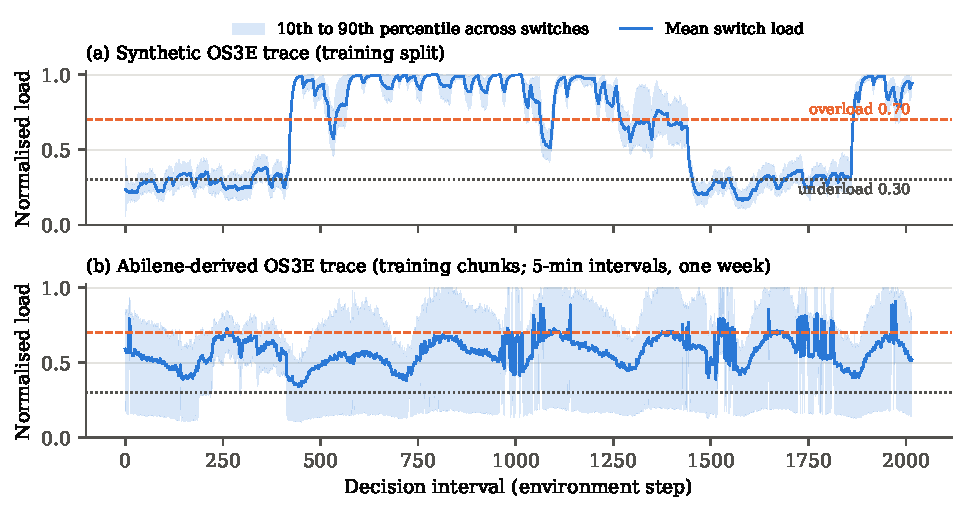
\includegraphics[width=\textwidth]{traffic_traces}
  \caption{Mean and 10th--90th percentile switch load over the first 2,016 steps of (a) the synthetic OS3E training split and (b) the Abilene-derived OS3E training split. Dashed and dotted lines mark the overload and underload thresholds.}
  \label{fig:traffic}
\end{figure}

\subsection{Abilene-derived real-traffic case study}
\label{sec:abilene}

To test the framework on measured traffic dynamics, the Abilene/Internet2 traffic-matrix archive~\cite{zhang2004abilene,zhang2003tm} was used. It provides $12\times12$ origin--destination (OD) matrices at 5-minute intervals in weekly chunks (\texttt{X01}--\texttt{X24}, 2,016 matrices each, 2004). Preprocessing (SHA-256 of the archive recorded) consists of four steps:
\begin{enumerate}[leftmargin=*]
  \item extract the measured OD component of each matrix and remove the diagonal;
  \item convert it to a 12-node load vector by summing each node's ingress and egress demand;
  \item project the 12 Abilene nodes onto the 34 OS3E switches with a fixed, documented two-source mapping (switch $i$ receives 0.80 of node $i \bmod 12$ and 0.20 of a second node);
  \item normalise each switch by the 99th percentile of the \emph{training} portion only, then clip to $[0,1]$.
\end{enumerate}
The result keeps the temporal structure of real backbone demand. It is \emph{not} measured OS3E traffic, and is referred to throughout as an \emph{Abilene-derived trace mapped to OS3E}.

Two isolated protocols were built from the archive:
\begin{itemize}[leftmargin=*]
  \item \textbf{Zero-shot transfer:} chunks \texttt{X06}--\texttt{X20} (30,240 steps) split 70/15/15. Only the 4,536-step test portion was used, to evaluate synthetic-trained OS3E models without any retraining.
  \item \textbf{Real-data training:} a fresh chunk-level split with training \texttt{X06}--\texttt{X14} (18,144 steps), validation \texttt{X15}--\texttt{X17} (6,048) and final test \texttt{X21}--\texttt{X24} (8,064). Chunks \texttt{X18}--\texttt{X20} were \emph{excluded} because they overlap the zero-shot evaluation window.
\end{itemize}
The real trace is markedly less stressed than the synthetic one. In the training data, 14\% of switch-load values exceed 0.70, against 59\% for synthetic OS3E (mean load 0.44 versus 0.70; Figure~\ref{fig:traffic}(b)).

\section{Implementation Details}
\label{sec:impl}

The framework was implemented in Python 3.10.14. Table~\ref{tab:software} lists the main libraries and Table~\ref{tab:modules} the modules. All training and evaluation ran on a CPU-only laptop (Intel Core~5~120U, 12 logical cores, 16\,GB RAM, Ubuntu 24.04); no GPU was used. Each run writes its checkpoint together with a JSON metadata file recording the state and action dimensions, hyperparameters, seed, traffic file, reward version (\path{normalized_multi_objective_v2}) and action-schema version (\path{stable_controller_slots_v2}). An evaluation refuses to load a checkpoint whose dimensions do not match the environment. Training was logged to TensorBoard, and evaluation results were written as CSV and JSON. A suite of eight unit tests (Appendix~\ref{app:verification}) checks the invariants that earlier bugs had violated, and all eight pass on the final code.

\begin{table}[htbp]
\centering
\caption{Software environment.}
\label{tab:software}
\small
\begin{tabular}{@{}ll@{}}
\toprule
\textbf{Component} & \textbf{Version / role}\\
\midrule
Python & 3.10.14\\
PyTorch~\cite{paszke2019pytorch} & 2.9.1 (CPU execution) -- Rainbow DQN and GRU\\
Gymnasium~\cite{towers2024gymnasium} & 1.2.3 -- environment interface\\
NetworkX~\cite{hagberg2008networkx} & 3.4.2 -- topology parsing, shortest paths, centrality\\
NumPy & 2.2.6 -- traffic generation and preprocessing\\
TensorBoard / Matplotlib & 2.20.0 / 3.10.8 -- logging and figures\\
\bottomrule
\end{tabular}
\end{table}

\begin{table}[htbp]
\centering
\caption{Main implementation modules.}
\label{tab:modules}
\small
\begin{tabularx}{\textwidth}{@{}P{6.4cm}L@{}}
\toprule
\textbf{Module} & \textbf{Responsibility}\\
\midrule
\path{utils/topology_loader.py} & GML parsing, haversine delays, shortest-path matrix, controller hosts\\
\path{experiments/preprocessing/create_synthetic_traffic.py} & Synthetic switch-load generator\\
\path{experiments/preprocessing/split_traffic_temporal.py} & Chronological 70/15/15 split with manifest\\
\path{experiments/preprocessing/prepare_abilene_*.py} & Abilene-to-OS3E projection and splits\\
\path{environments/threshold_proactive_sdn_env.py} & Environment: state, valid actions, feasibility, reward, metrics\\
\path{environments/rainbow_dqn_model.py} & Noisy dueling C51 network, PER, $n$-step buffer, projection, update\\
\path{forecasting/gru_traffic_predictor.py} & GRU network and frozen inference wrapper\\
\path{experiments/train_rainbow_fixed_rewards.py} & RDQN training (current/predictive), checkpoint metadata\\
\path{experiments/train_gru_forecaster.py} & GRU training, early stopping, persistence comparison\\
\path{experiments/evaluate_fair_baselines.py} & Identical-condition evaluation of RDQN and baselines\\
\path{experiments/evaluate_real_traffic_zero_shot.py} & Evaluation on an explicitly supplied real-derived trace\\
\path{tests/test_sdn_core.py} & Regression tests of environment and Rainbow invariants\\
\bottomrule
\end{tabularx}
\end{table}

\section{Experimental Settings}
\label{sec:settings}

\paragraph{Hyperparameters.} Table~\ref{tab:hyper} gives the Rainbow settings. Capacity scales with topology size, and the values were fixed before the final experiments. Common settings are $\gamma=0.99$, 51 atoms on $[-10,10]$, Adam, $\varepsilon$ decaying from 0.10 to 0.01 (time constant $0.6T$), one update per four steps after 1,000 warm-up steps, a target copy every 1,000 steps and 1,000-step training episodes.

\begin{table}[htbp]
\centering
\caption{Topology-dependent Rainbow DQN hyperparameters and recorded CPU training time.}
\label{tab:hyper}
\small
\fitwidth{\begin{tabular}{@{}lccccccc@{}}
\toprule
\textbf{Topology} & \textbf{Hidden $H$} & \textbf{LR} & \textbf{$n$} & \textbf{Batch} & \textbf{Buffer} & \textbf{Steps} & \textbf{Time (min)}\\
\midrule
Gridnet    & 128 & $2\times10^{-4}$ & 3 & 64  & 30k  & 80k  & 31.4 / 44.7\\
BellCanada & 256 & $1\times10^{-4}$ & 3 & 128 & 50k  & 80k  & 56.4 / 77.9\\
OS3E       & 256 & $1\times10^{-4}$ & 3 & 128 & 50k  & 80k  & 48.1 / 69.8\\
Interoute  & 512 & $5\times10^{-5}$ & 5 & 256 & 100k & 80k  & 143.0 / --\\
Cogentco   & 512 & $5\times10^{-5}$ & 5 & 256 & 100k & 80k, 120k & 222.8, 313.8 / --\\
\bottomrule
\end{tabular}}
\par\smallskip\footnotesize Time is current / predictive mode for the synthetic models. Real-data OS3E models took about 40\,min (current) and 50--52\,min (predictive) per seed.
\end{table}

\paragraph{Evaluation protocol.} A single evaluator runs every policy with the same topology, trace split, thresholds, reward, seed and evaluation windows. Each evaluation uses six episodes of 500 steps (3,000 decisions per policy), with start indices spread evenly across the split, $\text{start}_e=\lfloor e(L-500)/5\rfloor$ for $e=0,\dots,5$. Windows never wrap around the end of the split. The learned policy acts greedily over valid actions with noise disabled, and no learning occurs during evaluation. Validation runs use evaluation seed 1042 and final tests use seed 2042; models are trained with seed 42 unless stated otherwise.

\paragraph{Model selection and test discipline.} Figure~\ref{fig:protocol} shows the workflow. All tuning decisions were made on validation data:
\begin{itemize}[leftmargin=*]
  \item predictive RDQN was trained only for the topologies where the GRU beat persistence;
  \item a horizon-3 GRU was tried for Gridnet and BellCanada;
  \item the observation mode was chosen per topology;
  \item Cogentco was retrained with 120k steps after its 80k model under-performed on validation.
\end{itemize}
The configurations were then frozen and each test split was evaluated once. The validation run of the 120k Cogentco model was not recorded before its test evaluation. That result therefore lacks a validation confirmation, which is noted as a limitation. Only one Cogentco checkpoint was ever evaluated on the test split, so no selection among test results took place. For the real-data study, the seed-42 configuration was frozen after validation and then replicated unchanged with seeds 43 and 44, retraining both the GRU and the RDQN.

\begin{figure}[htbp]
  \centering
  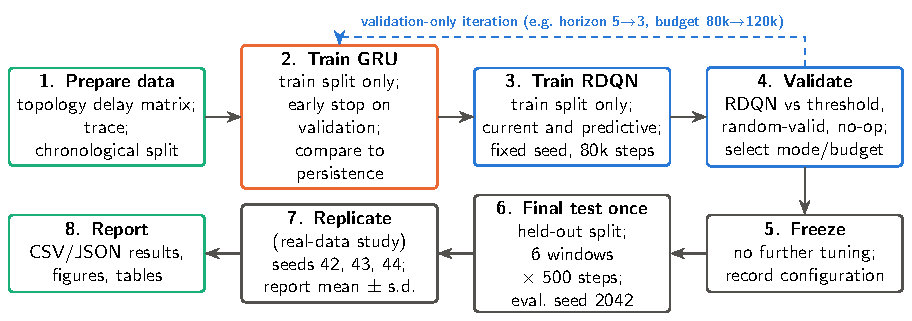
\includegraphics[width=\textwidth]{protocol}
  \caption{Experimental workflow. Iteration (dashed) used validation data only; each test split was used once, after freezing.}
  \label{fig:protocol}
\end{figure}

\begin{table}[htbp]
\centering
\caption{Summary of the three experimental protocols.}
\label{tab:protocols}
\small
\begin{tabularx}{\textwidth}{@{}p{3.0cm}LLL@{}}
\toprule
 & \textbf{Synthetic (E1)} & \textbf{Zero-shot real (E2)} & \textbf{Real-data-trained (E3)}\\
\midrule
Topologies & All five & OS3E & OS3E\\
Training traffic & Synthetic train split & Synthetic (no retraining) & Abilene \texttt{X06}--\texttt{X14}\\
Selection traffic & Synthetic validation split & -- & Abilene \texttt{X15}--\texttt{X17}\\
Test traffic & Synthetic test split & Abilene \texttt{X06}--\texttt{X20} test 15\% & Abilene \texttt{X21}--\texttt{X24}\\
Modes & Selected per topology & Current and predictive & Current and predictive\\
Training seeds & 42 & 42 & 42, 43, 44\\
Evaluation & $6\times500$, seed 2042 & $6\times500$, seed 2042 & $6\times500$, seed 2042\\
\bottomrule
\end{tabularx}
\end{table}

\section{Evaluation Criteria and Performance Metrics}
\label{sec:metrics}

Metrics are recorded at every evaluation step and aggregated as in Table~\ref{tab:metrics}. Cumulative reward is the primary criterion because it is the objective the agent optimises and it combines all three costs. Individual metrics are reported alongside it so that trade-offs are visible: a policy can improve the reward while losing on one metric. Rewards are comparable only within one protocol and observation mode, because the traffic and valid action sets differ between them.

\begin{table}[htbp]
\centering
\caption{Performance metrics.}
\label{tab:metrics}
\small
\begin{tabularx}{\textwidth}{@{}p{3.6cm}L@{}}
\toprule
\textbf{Metric} & \textbf{Definition (direction)}\\
\midrule
Cumulative reward & Sum of $r_t$ over a 500-step episode, averaged over six episodes (higher is better)\\
Average latency & Mean over switches of $D_{i,m(i)}$, averaged over steps (ms, lower)\\
Worst-case latency & Maximum assigned switch--controller delay in an episode, averaged over episodes (ms, lower)\\
Energy & Mean controller-state energy $E_t$ (W, lower)\\
Load index & Standard deviation of the number of switches per active controller (lower is more even)\\
Traffic balance & Coefficient of variation of active-controller loads (lower)\\
Overload / underload \% & Share of steps with at least one controller above 0.70 / below 0.30 before acting (lower)\\
Action counts, failures & Successful park, evoke and migrate actions per episode; failed actions\\
Forecast MAE & $\frac1N\lVert\hat{\mathbf{x}}_{t+h}-\mathbf{x}_{t+h}\rVert_1$ during evaluation (predictive mode)\\
Forecast-only actions & Successful evoke/migrate actions taken when overload was forecast but not current\\
GRU quality & Validation MAE, RMSE and overload F1 versus the persistence forecast\\
\bottomrule
\end{tabularx}
\end{table}

\chapter{Results and Discussion}
\label{ch:results}

This chapter reports the final held-out results of the three protocols (E1--E3, Table~\ref{tab:protocols}), compares the approach with existing methods, presents ablations and supporting analyses, and discusses what the evidence does and does not show. Unless stated otherwise, values are means over the six evaluation episodes; reward is per 500-step episode. Complete tables, including action counts, are given in Appendix~\ref{app:tables}.

\section{Overall Experimental Results}
\label{sec:overall}

\subsection{Training behaviour}

Figure~\ref{fig:training} shows the reward of every 1,000-step training episode for the selected synthetic models. The curves do not rise smoothly. Each training episode replays a different chronological window of the training trace, and the windows differ greatly in difficulty: a window that falls in a sustained peak cannot score as well as one in a quiet period, whatever the policy does. Training reward therefore mostly reflects the traffic window. It is not used here as evidence of learning; that evidence comes from comparing policies on identical held-out windows. The curves confirm that training was numerically stable, with no divergence or collapse, on every topology including the 197-switch Cogentco network.

\begin{figure}[htbp]
  \centering
  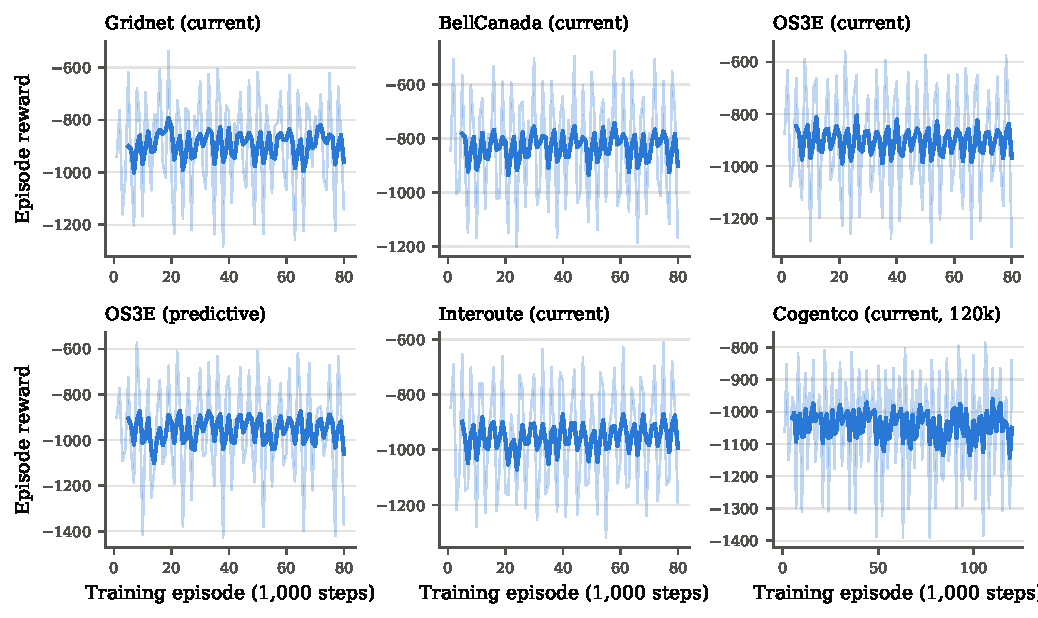
\includegraphics[width=\textwidth]{training_curves}
  \caption{Training-episode reward (light) and five-episode moving average (dark) for the selected synthetic models. Variation is dominated by the traffic window replayed in each episode.}
  \label{fig:training}
\end{figure}

\subsection{GRU forecasting quality}
\label{sec:res-gru}

Table~\ref{tab:gru} and Figure~\ref{fig:gru} compare the GRU forecasters with the persistence baseline on validation data. At horizon 5 the GRU reduced MAE by 15.6\% on Gridnet, 7.8\% on BellCanada and 8.5\% on OS3E, but was \emph{worse} than persistence on the two largest topologies (Interoute $-5.6$\%, Cogentco $-12.2$\%). Their traces are smoother, which makes persistence a strong forecaster, and one 64-unit GRU must model 110 and 197 correlated series. Predictive RDQN was therefore trained only for Gridnet, BellCanada and OS3E. Shortening the horizon to 3 improved Gridnet clearly but gave BellCanada almost no advantage over persistence. On the Abilene-derived trace the GRU had a slightly higher MAE than persistence but a lower RMSE and a higher overload F1 in all three seeds. In other words, it makes fewer large errors and detects more overload events, which is the property that matters for proactive decisions.

\begin{table}[htbp]
\centering
\caption{GRU forecaster versus persistence on validation data (history 12). Overload F1 is for predicting a switch load above 0.70. Bold marks the better of the pair.}
\label{tab:gru}
\small
\begin{tabular}{@{}llcccccc@{}}
\toprule
& & \multicolumn{2}{c}{\textbf{MAE}} & \multicolumn{2}{c}{\textbf{RMSE}} & \multicolumn{2}{c}{\textbf{Overload F1}}\\
\cmidrule(lr){3-4}\cmidrule(lr){5-6}\cmidrule(lr){7-8}
\textbf{Data} & \textbf{$h$} & GRU & Persist. & GRU & Persist. & GRU & Persist.\\
\midrule
Gridnet (syn.)    & 5 & \textbf{0.0345} & 0.0409 & \textbf{0.0487} & 0.0579 & \textbf{0.939} & 0.923\\
BellCanada (syn.) & 5 & \textbf{0.0360} & 0.0390 & \textbf{0.0504} & 0.0570 & \textbf{0.966} & 0.961\\
OS3E (syn.)       & 5 & \textbf{0.0356} & 0.0389 & \textbf{0.0537} & 0.0573 & \textbf{0.968} & 0.966\\
Interoute (syn.)  & 5 & 0.0370 & \textbf{0.0351} & 0.0561 & \textbf{0.0526} & 0.973 & \textbf{0.974}\\
Cogentco (syn.)   & 5 & 0.0361 & \textbf{0.0322} & 0.0549 & \textbf{0.0501} & 0.979 & \textbf{0.981}\\
\midrule
Gridnet (syn.)    & 3 & \textbf{0.0254} & 0.0299 & \textbf{0.0346} & 0.0411 & \textbf{0.953} & 0.944\\
BellCanada (syn.) & 3 & \textbf{0.0277} & 0.0278 & \textbf{0.0390} & 0.0397 & \textbf{0.974} & 0.972\\
\midrule
OS3E Abilene, seed 42 & 5 & 0.0294 & \textbf{0.0275} & \textbf{0.0416} & 0.0438 & \textbf{0.777} & 0.764\\
OS3E Abilene, seed 43 & 5 & 0.0294 & \textbf{0.0275} & \textbf{0.0424} & 0.0438 & \textbf{0.768} & 0.764\\
OS3E Abilene, seed 44 & 5 & 0.0296 & \textbf{0.0275} & \textbf{0.0424} & 0.0438 & \textbf{0.779} & 0.764\\
\bottomrule
\end{tabular}
\end{table}

\begin{figure}[htbp]
  \centering
  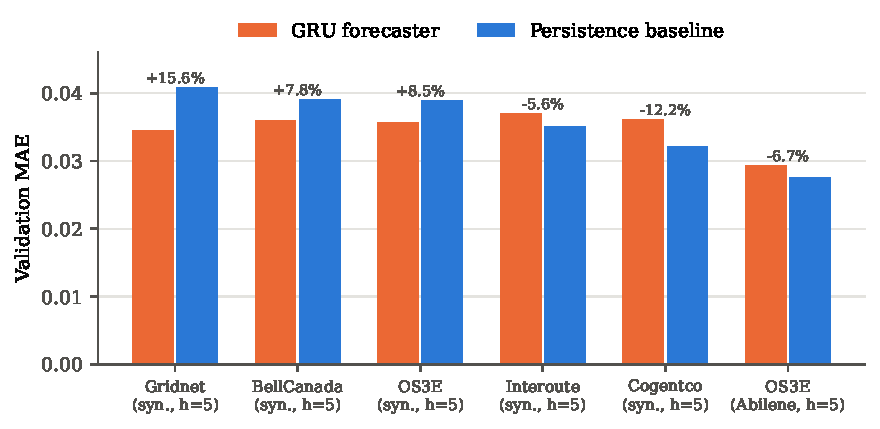
\includegraphics[width=0.92\textwidth]{gru_vs_persistence}
  \caption{Validation MAE of the GRU and the persistence forecast (horizon 5). Labels give the GRU's relative MAE improvement; negative values mean persistence is better.}
  \label{fig:gru}
\end{figure}

\subsection{E1: Synthetic held-out results across five topologies}
\label{sec:res-syn}

Table~\ref{tab:syn-main} reports the final test results for the selected learned policy of each topology against the three baselines evaluated under the same conditions. Figures~\ref{fig:syn-reward} and~\ref{fig:syn-metrics} show the same comparison graphically. The selected policy is current-state RDQN for four topologies and predictive GRU-RDQN for OS3E, following validation (Section~\ref{sec:ablation-mode}).

\begin{table}[htbp]
\centering
\caption{E1 final test on held-out synthetic traffic: selected learned policy versus baselines (six episodes $\times$ 500 steps, evaluation seed 2042). Best value per topology and metric in bold.}
\label{tab:syn-main}
\small
\fitwidth{\begin{tabular}{@{}llrrrrr@{}}
\toprule
\textbf{Topology} & \textbf{Policy} & \textbf{Reward}$\uparrow$ & \textbf{Avg lat.}$\downarrow$ & \textbf{Worst lat.}$\downarrow$ & \textbf{Energy}$\downarrow$ & \textbf{Load idx}$\downarrow$\\
 & & & (ms) & (ms) & (W) & \\
\midrule
\multirow{4}{*}{Gridnet} & Current RDQN & \textbf{$-$446.33} & 8.81 & 20.78 & 411.67 & 0.919\\
 & Threshold & $-$474.97 & 7.98 & 21.37 & 429.73 & 0.906\\
 & Random-valid & $-$464.30 & 8.23 & 21.09 & 423.13 & 0.922\\
 & No-op & $-$505.82 & \textbf{3.68} & \textbf{12.85} & \textbf{370.00} & \textbf{0.816}\\
\midrule
\multirow{4}{*}{BellCanada} & Current RDQN & \textbf{$-$384.27} & 11.51 & 34.86 & 398.11 & \textbf{6.162}\\
 & Threshold & $-$408.54 & 11.15 & 36.27 & 446.56 & 6.337\\
 & Random-valid & $-$424.66 & 11.63 & 33.16 & 447.85 & 6.216\\
 & No-op & $-$529.37 & \textbf{10.70} & \textbf{25.28} & \textbf{370.00} & 14.236\\
\midrule
\multirow{4}{*}{OS3E} & Predictive GRU-RDQN & \textbf{$-$452.94} & 4.54 & 15.89 & 380.89 & 4.223\\
 & Threshold (pred.) & $-$508.53 & 4.15 & 15.76 & 445.60 & \textbf{3.637}\\
 & Random-valid (pred.) & $-$515.07 & 4.54 & 15.76 & 447.22 & 4.403\\
 & No-op & $-$507.38 & \textbf{2.60} & \textbf{11.51} & \textbf{370.00} & 4.190\\
\midrule
\multirow{4}{*}{Interoute} & Current RDQN & \textbf{$-$477.57} & 6.01 & 17.38 & 383.38 & 19.353\\
 & Threshold & $-$529.96 & 5.79 & 17.38 & 461.02 & 18.709\\
 & Random-valid & $-$528.67 & 5.25 & 16.33 & 461.20 & 18.389\\
 & No-op & $-$499.02 & \textbf{4.39} & \textbf{14.57} & \textbf{370.00} & \textbf{18.117}\\
\midrule
\multirow{4}{*}{Cogentco} & Current RDQN (120k) & \textbf{$-$447.52} & 15.18 & 51.05 & 373.54 & 37.957\\
 & Threshold & $-$514.59 & 16.18 & 51.67 & 464.35 & 39.063\\
 & Random-valid & $-$522.46 & 15.96 & 57.01 & 463.33 & 37.305\\
 & No-op & $-$472.06 & \textbf{7.59} & \textbf{29.79} & \textbf{370.00} & \textbf{34.922}\\
\bottomrule
\end{tabular}}
\end{table}

\begin{figure}[htbp]
  \centering
  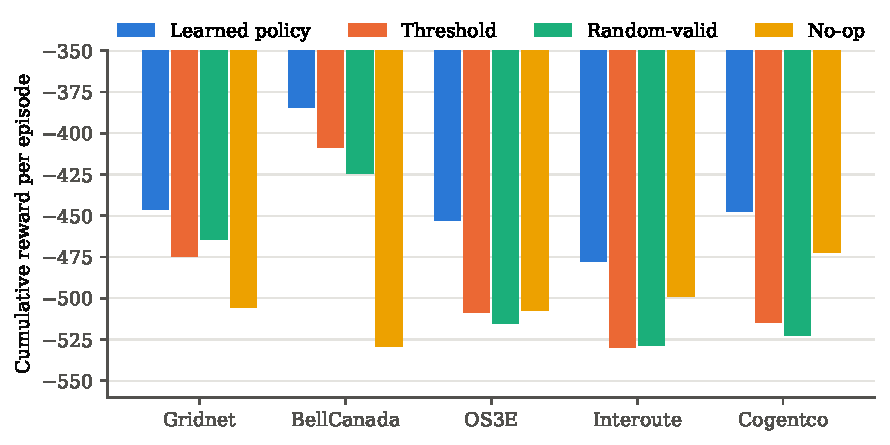
\includegraphics[width=\textwidth]{syn_reward}
  \caption{E1 final-test cumulative reward per episode (higher is better). The learned policy is current RDQN except for OS3E (predictive GRU-RDQN).}
  \label{fig:syn-reward}
\end{figure}

\begin{figure}[htbp]
  \centering
  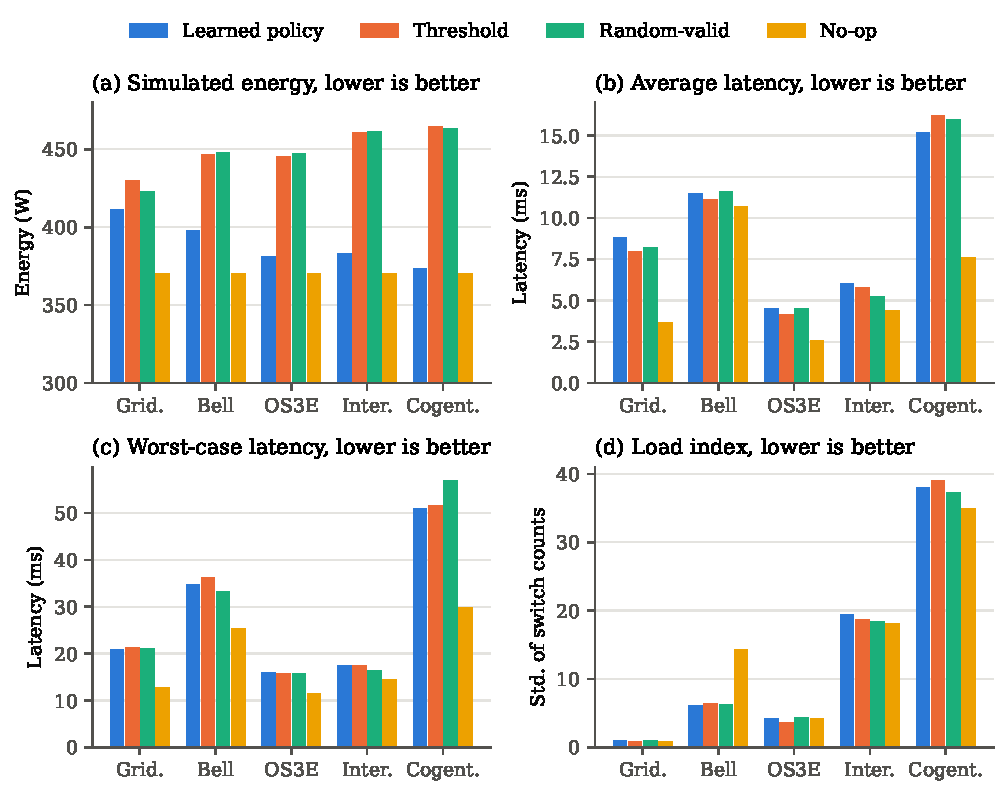
\includegraphics[width=\textwidth]{syn_metrics}
  \caption{E1 final-test operating metrics for the same policies as Figure~\ref{fig:syn-reward}.}
  \label{fig:syn-metrics}
\end{figure}

\paragraph{Principal finding.} The learned policy obtained the \textbf{highest reward on all five topologies}, ahead of all three baselines. Table~\ref{tab:syn-delta} expresses the result relative to the threshold policy, the strongest practical baseline. The learned policy consistently used less energy, from 18\,W (4.2\%) on Gridnet up to 91\,W (19.6\%) on Cogentco, and the saving grows with topology size. It achieved this mainly by keeping fewer controllers active: on Interoute and Cogentco its mean energy (383 and 374\,W) is close to the 370\,W of the initial three-controller state, whereas the threshold policy averaged more than 460\,W because it evokes whenever overload appears.

\begin{table}[htbp]
\centering
\caption{E1: change of the learned policy relative to the threshold baseline (learned minus threshold). Positive reward and negative energy/latency are improvements.}
\label{tab:syn-delta}
\small
\fitwidth{\begin{tabular}{@{}lrrrrr@{}}
\toprule
\textbf{Topology} & \textbf{$\Delta$Reward} & \textbf{$\Delta$Energy (W)} & \textbf{$\Delta$Avg lat. (ms)} & \textbf{$\Delta$Worst lat. (ms)} & \textbf{$\Delta$Load idx}\\
\midrule
Gridnet          & $+28.64$ & $-18.06$ ($-4.2$\%)  & $+0.83$ & $-0.59$ & $+0.013$\\
BellCanada       & $+24.27$ & $-48.45$ ($-10.8$\%) & $+0.36$ & $-1.41$ & $-0.175$\\
OS3E (predictive)& $+55.59$ & $-64.71$ ($-14.5$\%) & $+0.39$ & $+0.13$ & $+0.586$\\
Interoute        & $+52.40$ & $-77.64$ ($-16.8$\%) & $+0.22$ & $\phantom{+}0.00$ & $+0.644$\\
Cogentco         & $+67.07$ & $-90.81$ ($-19.6$\%) & $-1.00$ & $-0.61$ & $-1.106$\\
\bottomrule
\end{tabular}}
\end{table}

\paragraph{Trade-offs.} The learned policy does not win on every metric. Its average latency was 0.2--0.8\,ms higher than the threshold policy's on four topologies; Cogentco is the exception, with 1.0\,ms lower. Its worst-case latency was lower or equal on four topologies. Its count-based load index was mixed. These trade-offs are intended by the design: the reward weights energy and traffic balance alongside latency, and parking a controller necessarily moves its switches to more distant controllers.

\paragraph{The no-op reference.} No-op has the lowest latency and energy in every topology, because it keeps the initial nearest-controller assignment and never evokes extra controllers. It never responds to overload, which is present in 55--69\% of steps on this traffic, and never parks controllers during quiet periods, so its low latency and energy are not good controller management. Its reward is the worst of all policies on Gridnet and BellCanada. On OS3E, Interoute and Cogentco, however, no-op ranks \emph{second}, ahead of both active baselines. On those topologies, reacting to every overload by evoking costs more energy than it recovers, and the learned policy's restraint (few evokes, near-baseline energy) is what pays off. The no-op results show why individual metrics must be read together with the reward, and why simple reactivity is not automatically better than inaction.

\paragraph{Uncertainty.} The standard deviation of episode reward \emph{within} each evaluation is large (about 145--225 for the learned policies), because the six windows differ in traffic intensity. All policies see the same six windows, so the comparison is paired. Only per-window aggregates were stored, however, so a formal paired test is not possible from the saved results, and the synthetic results come from a single training seed. The margins over the threshold policy (24--67 reward points) are consistent in direction across five independent topologies, which supports the finding, but they are not a statistical significance claim.

\subsection{E2: Zero-shot transfer to Abilene-derived traffic}
\label{sec:res-zeroshot}

E2 tests whether the synthetic-trained OS3E policies still behave sensibly on real traffic dynamics they have never seen. Table~\ref{tab:zeroshot} and Figure~\ref{fig:zeroshot} give the results. In both modes the learned policy had the best reward and the lowest energy of all active policies. Predictive GRU-RDQN was marginally better than current RDQN on reward ($-74.62$ versus $-76.56$), energy ($-3.8$\,W), worst-case latency ($-0.63$\,ms) and load index (0.986 versus 1.548). The differences are small. Overload occurs in less than 1\% of steps on this trace, so the policies mainly had to decide when to park. The GRU's forecast error rose from 0.037 on synthetic OS3E to 0.176 here, a clear sign of distribution shift. E2 therefore shows that the policies \emph{transfer without failure}: they produce zero failed actions and still beat the baselines. It does not show that prediction generalises.

\begin{table}[htbp]
\centering
\caption{E2 zero-shot results on the Abilene-derived OS3E test trace (models trained on synthetic OS3E only).}
\label{tab:zeroshot}
\small
\fitwidth{\begin{tabular}{@{}llrrrrrr@{}}
\toprule
\textbf{Mode} & \textbf{Policy} & \textbf{Reward} & \textbf{Avg lat.} & \textbf{Worst lat.} & \textbf{Energy} & \textbf{Load idx} & \textbf{Under\%}\\
\midrule
\multirow{4}{*}{Current} & RDQN & \textbf{$-$76.56} & 6.45 & 18.14 & \textbf{218.65} & \textbf{1.548} & \textbf{9.8}\\
 & Threshold & $-$82.27 & 6.41 & 18.14 & 231.79 & 1.757 & 10.4\\
 & Random-valid & $-$82.44 & 6.22 & 17.51 & 229.21 & 2.238 & 10.3\\
 & No-op & $-$233.34 & 2.60 & 11.51 & 370.00 & 4.190 & 28.2\\
\midrule
\multirow{4}{*}{Predictive} & GRU-RDQN & \textbf{$-$74.62} & 6.39 & 17.51 & \textbf{214.81} & \textbf{0.986} & \textbf{10.1}\\
 & Threshold & $-$83.44 & 6.38 & 18.14 & 233.32 & 1.619 & 10.5\\
 & Random-valid & $-$90.73 & 6.45 & 18.14 & 235.06 & 2.477 & 11.3\\
 & No-op & $-$233.34 & 2.60 & 11.51 & 370.00 & 4.190 & 28.2\\
\bottomrule
\end{tabular}}
\par\smallskip\footnotesize Forecast MAE in predictive mode: 0.1764. Overload occurred in at most 0.6\% of steps for any policy.
\end{table}

\begin{figure}[htbp]
  \centering
  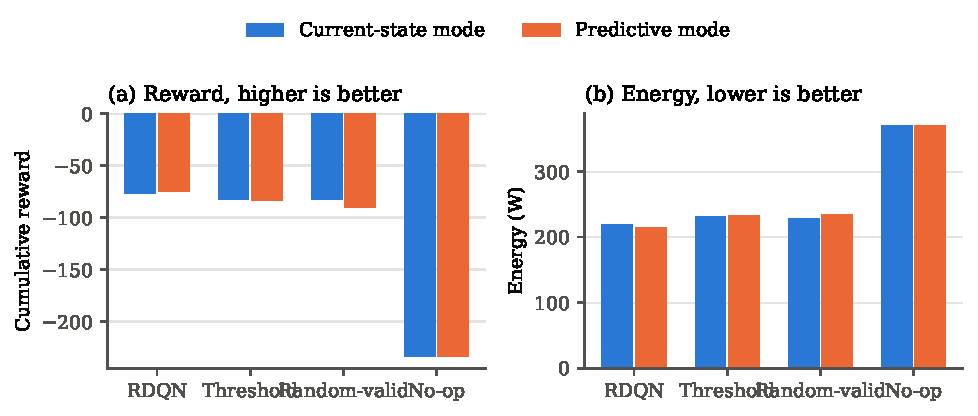
\includegraphics[width=0.95\textwidth]{zero_shot}
  \caption{E2 zero-shot reward and energy on the Abilene-derived OS3E test trace, by policy and observation mode.}
  \label{fig:zeroshot}
\end{figure}

\subsection{E3: Real-data-trained OS3E with three training seeds}
\label{sec:res-real}

In E3 the GRU, current RDQN and predictive GRU-RDQN were trained on Abilene-derived data and tested on the untouched final weeks \texttt{X21}--\texttt{X24}. The procedure was repeated for seeds 42, 43 and 44. Table~\ref{tab:real-agg} reports mean $\pm$ sample standard deviation, Table~\ref{tab:real-seed} reports the per-seed rewards, and Figure~\ref{fig:real} shows both.

\begin{table}[htbp]
\centering
\caption{E3 final test, mean $\pm$ sample s.d. across training seeds 42, 43 and 44. Both models had zero failed actions in every run.}
\label{tab:real-agg}
\small
\begin{tabular}{@{}lrr@{}}
\toprule
\textbf{Metric} & \textbf{Current RDQN} & \textbf{Predictive GRU-RDQN}\\
\midrule
Reward $\uparrow$ & $-121.80\pm20.14$ & $\mathbf{-111.19\pm17.53}$\\
Average latency (ms) $\downarrow$ & $\mathbf{5.57\pm0.01}$ & $5.70\pm0.24$\\
Worst-case latency (ms) $\downarrow$ & $17.12\pm0.13$ & $17.12\pm0.15$\\
Energy (W) $\downarrow$ & $270.98\pm2.78$ & $\mathbf{269.18\pm5.48}$\\
Load index $\downarrow$ & $\mathbf{3.19\pm0.76}$ & $3.45\pm0.48$\\
Overload steps (\%) $\downarrow$ & $10.03\pm3.26$ & $\mathbf{8.01\pm1.97}$\\
Underload steps (\%) $\downarrow$ & $10.24\pm2.33$ & $\mathbf{8.64\pm2.40}$\\
\bottomrule
\end{tabular}
\end{table}

\begin{table}[htbp]
\centering
\caption{E3 per-seed final-test reward of each learned policy and its same-mode threshold baseline.}
\label{tab:real-seed}
\small
\begin{tabular}{@{}lrrrr@{}}
\toprule
& \multicolumn{2}{c}{\textbf{Current mode}} & \multicolumn{2}{c}{\textbf{Predictive mode}}\\
\cmidrule(lr){2-3}\cmidrule(lr){4-5}
\textbf{Seed} & RDQN & Threshold & GRU-RDQN & Threshold\\
\midrule
42 & \textbf{$-$107.39} & $-$127.32 & \textbf{$-$122.71} & $-$166.31\\
43 & \textbf{$-$113.20} & $-$127.32 & $-$119.84 & \textbf{$-$117.66}\\
44 & $-$144.82 & \textbf{$-$127.32} & \textbf{$-$91.02} & $-$117.41\\
\midrule
Mean & \textbf{$-$121.80} & $-$127.32 & \textbf{$-$111.19} & $-$133.79\\
\bottomrule
\end{tabular}
\par\smallskip\footnotesize The current-mode threshold is identical across seeds because it does not depend on any trained model; the predictive-mode threshold depends on each seed's GRU through the valid-action set.
\end{table}

\begin{figure}[htbp]
  \centering
  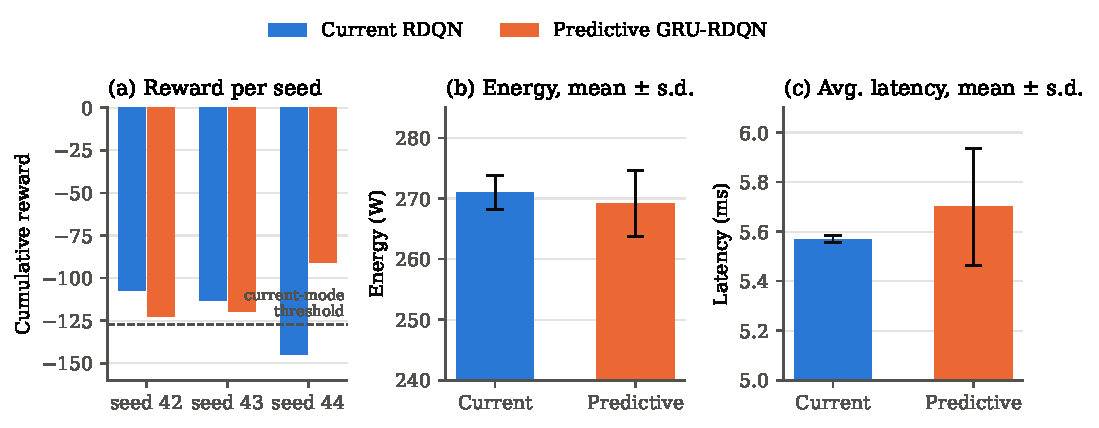
\includegraphics[width=\textwidth]{real_three_seed}
  \caption{E3 final test. (a) Reward of each seed; the dashed line is the current-mode threshold. (b, c) Mean $\pm$ sample s.d. of energy and average latency (axes truncated to show the differences).}
  \label{fig:real}
\end{figure}

Averaged over seeds, predictive GRU-RDQN achieved a better reward ($+10.61$), slightly lower energy ($-1.8$\,W) and fewer overload and underload steps. Current RDQN kept slightly lower average latency ($-0.13$\,ms) and a lower load index, and worst-case latency was identical. The per-seed results, however, show that the predictive advantage in mean reward comes from \emph{one} seed. Current RDQN was better for seeds 42 and 43, by 15.3 and 6.6 points, and predictive GRU-RDQN was better for seed 44, by 53.8 points. The between-seed standard deviations (about 18--20 points) exceed the mean difference. With three seeds, the honest conclusion is that the two modes are \emph{not distinguishable} on this trace. On average, each learned policy beat its same-mode threshold baseline: by 5.5 points in current mode and 22.6 in predictive mode. They did not do so on every seed, since current RDQN lost to threshold for seed 44 and predictive GRU-RDQN lost narrowly for seed 43.

Validation for E3 (Appendix~\ref{app:tables}) took place in an almost overload-free period ($\le0.2$\% of steps) in which all active policies were within about 2.5 reward points of each other. That validation period could not separate the models, and this probably contributes to the seed-to-seed variability of the selected checkpoints.

\section{Comparison with Existing Methods}
\label{sec:compare-existing}

The baselines in this study are threshold, random-valid and no-op policies implemented in the same environment; published algorithms were not re-implemented. A direct numerical comparison with published results is not valid, for three reasons:
\begin{enumerate}[leftmargin=*]
  \item The \emph{decision problems} differ. MOOO-RDQN~\cite{chen2025mooo}, DDCP~\cite{bouzidi2022ddcp} and AP-DQN~\cite{farahi2026apdqn} choose placements; SAR-LB~\cite{yeo2021sarlb} migrates among a fixed set of controllers; Li \emph{et al.}~\cite{li2024mec} place controllers and select edges in MEC.
  \item The \emph{traffic, controller counts and capacities} differ.
  \item The \emph{metrics} differ: those papers report percentage improvements over their own baselines, whereas this work reports a bounded reward together with absolute latency and modelled energy.
\end{enumerate}
For the same reason, latency and load values transcribed from the MOOO-RDQN paper into an early evaluation script were deliberately excluded from this report. They could not be verified and they measure a placement outcome, not a runtime policy.

The comparison that can be made is methodological (Table~\ref{tab:litcompare}). Relative to that literature, the distinctive elements of this work are listed below.
\begin{itemize}[leftmargin=*]
  \item \textbf{Joint runtime actions.} One policy chooses migrate, park, evoke or wait. The E1 results show the value of this combination: most of the learned policy's advantage over threshold control comes from \emph{energy}, which a migration-only policy such as SAR-LB cannot change, while overload is still handled through migration.
  \item \textbf{A matched forecast ablation.} Unlike forecast-assisted placement~\cite{li2024mec}, the same agent is trained with and without forecasts, which shows that the forecast's value depends on the topology and the traffic.
  \item \textbf{Evaluation discipline.} The study uses chronological splits, a single-use test set, baselines run under identical conditions, a zero-shot transfer test and multi-seed replication, as recommended for credible DRL evaluation~\cite{henderson2018matters,agarwal2021precipice}.
\end{itemize}
Conversely, those works include elements not covered here: controller placement itself, a real controller platform (ONOS in DDCP), formal safety layers~\cite{dinh2025safe} and multi-domain federated training~\cite{jha2026federated}.

\section{Ablation Studies and Additional Analyses}
\label{sec:ablation}

\subsection{Current-state versus predictive observation}
\label{sec:ablation-mode}

The main ablation removes the forecast input while keeping everything else identical: environment, reward, network, seed and budget. Table~\ref{tab:ablation-mode} shows the synthetic validation results that determined the observation mode for each topology.

\begin{table}[htbp]
\centering
\caption{Ablation on synthetic validation data: current RDQN versus predictive GRU-RDQN (horizons 5 and 3). Rewards in predictive mode are compared with the best predictive-mode baseline.}
\label{tab:ablation-mode}
\small
\fitwidth{\begin{tabular}{@{}llrrrrr@{}}
\toprule
\textbf{Topology} & \textbf{Model} & \textbf{Reward} & \textbf{Avg lat.} & \textbf{Energy} & \textbf{Load idx} & \textbf{F.-only acts}\\
\midrule
\multirow{3}{*}{Gridnet} & Current RDQN & \textbf{$-$440.90} & 8.81 & \textbf{411.31} & \textbf{0.807} & --\\
 & Predictive, $h=5$ & $-$493.40 & \textbf{8.02} & 418.78 & 1.072 & 2.67\\
 & Predictive, $h=3$ & $-$491.91 & 8.70 & 413.50 & 0.986 & --\\
\midrule
\multirow{3}{*}{BellCanada} & Current RDQN & \textbf{$-$399.99} & 11.74 & \textbf{405.85} & 8.405 & --\\
 & Predictive, $h=5$ & $-$441.32 & \textbf{11.25} & 439.45 & \textbf{7.316} & 2.50\\
 & Predictive, $h=3$ & $-$437.84 & 11.79 & 441.49 & 7.940 & --\\
\midrule
\multirow{2}{*}{OS3E} & Current RDQN & $-$480.22 & 5.12 & 441.19 & 3.729 & --\\
 & Predictive, $h=5$ & \textbf{$-$445.81} & \textbf{4.39} & \textbf{383.83} & \textbf{3.653} & 5.67\\
\bottomrule
\end{tabular}}
\par\smallskip\footnotesize ``F.-only acts'': successful actions per episode taken on forecast-only overload. Best predictive baselines on validation: Gridnet $-$513.55, BellCanada $-$462.27 ($h=5$) / $-$438.92 ($h=3$), OS3E $-$493.56.
\end{table}

On OS3E, prediction improved \emph{every} metric on validation. The predictive agent also used forecast-only actions most often there (5.67 per episode), and the improvement carried over to the final test, where predictive GRU-RDQN scored $-452.94$ against $-478.46$ for current RDQN and used 380.89\,W against 442.18\,W. Notably, current RDQN on OS3E had \emph{not} beaten the threshold policy ($-478.46$ versus $-474.79$ on test), so OS3E is the topology where forecasting made the difference between a learned policy that beats threshold control and one that does not. On Gridnet and BellCanada, prediction improved latency but lowered reward and raised energy compared with current RDQN, although it still beat every predictive-mode baseline. Mode comparisons across tables should be read with care, because predictive mode changes the valid-action sets and therefore the baselines' trajectories. The within-mode comparison is the strictly fair one.

\subsection{Forecast horizon}

Reducing the horizon from 5 to 3 (Table~\ref{tab:ablation-mode}) slightly improved predictive reward on Gridnet ($-493.40\rightarrow-491.91$) and BellCanada ($-441.32\rightarrow-437.84$), consistent with the more accurate horizon-3 forecasts (Table~\ref{tab:gru}). It did not close the gap to current RDQN, so horizon 5 was kept for OS3E and current mode was selected for Gridnet and BellCanada.

\subsection{Training budget on the largest topology}

With 80k steps, Cogentco current RDQN \emph{lost} on validation to no-op ($-538.46$ versus $-481.67$) and to threshold ($-524.98$), and used 452\,W. Retrained with 120k steps, it won on the final test ($-447.52$ against $-472.06$ for no-op) and used 374\,W, with fewer evokes (1.5 versus 2.7 per episode). The two numbers come from different splits, so they are not a controlled comparison. They are, however, consistent with the expectation that a 208-action problem needs more experience. Cogentco's training time (314\,min for 120k steps on CPU) also shows the cost of scaling a flat action space.

\subsection{Action behaviour and validity}

Across all reported final tests, both learned and baseline policies had \textbf{zero failed actions}, which confirms that the valid-action mask and feasibility checks work as intended. On synthetic traffic the learned policies performed 1.7--2.8 parks, 1.5--3.2 evokes and 24--57 migrations per 500-step episode, and took no action in the remaining 87--95\% of steps (Appendix~\ref{app:tables}). Compared with threshold control, they evoked less often on the large topologies; on Interoute, 1.7 versus 2.8 evokes per episode with fewer migrations, which explains most of the energy difference. The policies therefore learned \emph{when not to add capacity}, a judgement a fixed rule cannot make.

\subsection{Implementation verification}

Before any final experiment, an audit of an earlier version of the code found twelve defects, summarised in Appendix~\ref{app:verification}. They included traffic advancing only every 50 steps, evaluation always starting at the low-load start of the trace, rewards of about $\pm200$ outside the C51 support, probability mass lost in the C51 projection, unflushed $n$-step returns and state-dependent action indices. All results in this chapter were produced after these fixes with new models; pre-fix results are not reported. Eight regression tests now guard these invariants.

\section{Discussion of Findings}
\label{sec:discussion}

\paragraph{Objective O1 (environment).} The environment reproduces the intended decision problem across five real topologies of very different size. Its valid-action mechanism eliminated failed actions for all policies, and its stable action schema and versioned checkpoints made results reproducible and kept incompatible models from being evaluated.

\paragraph{Objective O2 (learning and fair evaluation).} On held-out synthetic traffic, Rainbow DQN learned controller-management policies that beat threshold, random-valid and no-op control in reward on all five topologies. The main mechanism is energy-aware restraint: keeping fewer controllers active, adding capacity only when it pays off, and still resolving overload by migration. The cost is a small increase in average latency on most topologies. This is the trade-off the reward was designed to make, not a defect, but a deployment that prioritises latency would need different weights.

\paragraph{Objective O3 (forecasting).} Forecasting helped where the forecaster was accurate \emph{and} the policy used it. OS3E had the most forecast-only actions and the largest gain. It did not help on Gridnet and BellCanada despite good forecasts, which suggests that the extra 15--54 state dimensions made learning harder within the same 80k-step budget. On real traffic the evidence was neutral: averaged over three seeds predictive mode was ahead, but one seed drove that difference. The answer to O3 is therefore conditional: \emph{a GRU forecast can make controller management more proactive and more energy-efficient, but its benefit depends on the topology, the forecast quality and the traffic regime, and it is not universal.}

\paragraph{Limitations and threats to validity.}
\begin{itemize}[leftmargin=*]
  \item \emph{Construct validity.} Latency is graph propagation delay only; queueing and controller processing delay are not modelled. Energy is a three-level state model. Controller capacity is represented by fixed normalised thresholds.
  \item \emph{External validity.} The synthetic generator, although stress-oriented and topology-scaled, is not operator traffic. The real-traffic study maps 12 Abilene nodes onto 34 OS3E switches through a fixed projection and covers one topology. No OpenFlow controller or Mininet deployment was used.
  \item \emph{Statistical validity.} The synthetic results use one training seed, and E3 uses three. Within-evaluation reward variance is large, and per-window results were not stored for paired testing. No significance claims are made.
  \item \emph{Internal validity.} Selection decisions used validation data only, and test splits were used once. The Cogentco 120k model lacks a recorded validation run, and E3 validation was too quiet to discriminate between models. The reward weights and thresholds were fixed by design and not tuned, and their sensitivity is untested.
  \item \emph{Scalability.} A separate agent is trained per topology, and the flat action space grows with $N$, which makes training on large networks expensive on CPU.
\end{itemize}
These limitations bound the claims made in this report. They do not undermine the central result, which rests on matched comparisons inside a single, documented environment.

\chapter{Conclusion}
\label{ch:conclusion}

\section{Summary of Research and Key Findings}

This research studied runtime controller management in distributed SDN as a sequential decision problem. A Rainbow DQN agent, acting as the master controller, observed controller loads, controller states and the switch mapping, optionally with GRU forecasts of near-future load. At each interval it chose to migrate a switch, park or evoke a controller, or do nothing. A valid-action mechanism kept every decision executable, and a bounded reward balanced latency, modelled energy and load balance. The framework was evaluated on five Topology Zoo networks of 9 to 197 switches, on synthetic and Abilene-derived traffic, against threshold, random-valid and no-op policies run under identical conditions, with chronological splits and single-use test sets.

The key findings are as follows.
\begin{enumerate}[leftmargin=*]
  \item On held-out synthetic traffic, the selected learned policy achieved the \textbf{highest reward on all five topologies} and used \textbf{4.2--19.6\% less simulated energy} than threshold control, with the saving growing with network size. The price was a small increase in average latency (0.2--0.8\,ms) on four of the five topologies.
  \item The gain comes mainly from \textbf{energy-aware restraint}. The agent learned to add controllers less often than a reactive rule and to park them when possible, while still relieving overload through migration. No failed actions occurred in any final evaluation.
  \item \textbf{Forecasting is scenario-dependent.} The GRU beat persistence on three of five synthetic topologies. Predictive GRU-RDQN clearly improved OS3E (reward $-478.46\rightarrow-452.94$, energy $442.18\rightarrow380.89$\,W relative to current RDQN), but not Gridnet or BellCanada.
  \item On \textbf{real traffic dynamics}, synthetic-trained policies transferred zero-shot without failures and still beat the baselines. After real-data training, the two modes could not be separated over three seeds (predictive mean reward $-111.19\pm17.53$ versus $-121.80\pm20.14$, with current RDQN better in two of three seeds).
  \item Larger topologies need larger training budgets: Cogentco required 120k rather than 80k steps.
\end{enumerate}

\section{Research Contributions}

\begin{enumerate}[leftmargin=*]
  \item \textbf{A runtime controller-management formulation} in which a single learned discrete policy jointly chooses switch migration, controller parking, controller evoking and no action, with a stable action schema, valid-action masking and feasibility checks.
  \item \textbf{A proactive extension with a controlled ablation}: a frozen GRU forecaster integrated conservatively, with forecasts allowed to anticipate overload but not to remove capacity or alter rewards, and evaluated against an otherwise identical current-state agent.
  \item \textbf{A leakage-controlled evaluation protocol and evidence across scales}: chronological splits, validation-only selection, single-use tests, identical-condition baselines, zero-shot transfer and three-seed real-data replication over five topologies.
  \item \textbf{Reproducible artefacts}: versioned checkpoints with metadata, CSV/JSON results, regression tests and scripts that regenerate every figure and table in this report from the stored results.
\end{enumerate}
The contribution lies in the integration and evaluation of these components; Rainbow DQN, GRU forecasting, switch migration and controller activation are each pre-existing techniques.

\section{Future Work}

\begin{itemize}[leftmargin=*]
  \item \textbf{Testbed validation.} Run the trained policies in Mininet~\cite{lantz2010mininet} with a distributed controller platform (e.g.\ ONOS or OpenDaylight) to measure real flow-setup latency, migration overhead and controller resource use.
  \item \textbf{Richer models.} Add queueing and processing delay and controller-specific capacities, and replace the three-level energy model with measured or empirically fitted power profiles.
  \item \textbf{Statistical strength.} Train every configuration with ten or more seeds, store per-window results and report paired tests with confidence intervals~\cite{agarwal2021precipice}.
  \item \textbf{Sensitivity and component ablations.} Vary the reward weights, thresholds and forecast horizons, and remove individual Rainbow components and the action mask, to measure their contribution.
  \item \textbf{Scalable, transferable policies.} Use graph neural network state encoders and factorised (switch, target) actions so that a single policy generalises across topologies, and explore federated multi-domain training~\cite{jha2026federated}.
  \item \textbf{Better forecasting and safety.} Use topology-aware forecasters for large networks, uncertainty-aware forecasts that the agent can weigh, and formal safety layers such as control barrier functions~\cite{dinh2025safe}.
\end{itemize}


% =====================================================================
%  REFERENCES (IEEE)
% =====================================================================
\renewcommand{\bibname}{References}
\IfFileExists{IEEEtran.bst}{\bibliographystyle{IEEEtran}}{\bibliographystyle{ieeetr}}
\bibliography{references}

% =====================================================================
%  APPENDICES
% =====================================================================
\appendix
\chapter{Complete Result Tables}
\label{app:tables}

The tables below are generated automatically from the frozen evaluation CSV files by \path{report/scripts/make_appendix_tables.py}. Each row is the mean over six evaluation episodes of 500 steps; ``s.d.'' is the standard deviation of episode reward \emph{across the six windows}, which mainly reflects differences in traffic intensity between windows. Park, Evoke and Mig are successful actions per episode, Fail is failed actions per episode, and Over\%/Under\% are the shares of steps with at least one overloaded/underloaded controller before acting. Validation runs use evaluation seed 1042 and final tests use seed 2042.

% AUTO-GENERATED by report/scripts/make_appendix_tables.py -- do not edit by hand.
\begin{table}[H]
\centering
\caption{E1 final test, current mode (Gridnet, BellCanada, OS3E, Interoute; 80k steps).}
\label{tab:app-e1-current}
\scriptsize
\setlength{\tabcolsep}{3pt}
\fitwidth{\begin{tabular}{@{}llrrrrrrrrrrrr@{}}
\toprule
\textbf{Topology} & \textbf{Policy} & \textbf{Reward} & \textbf{s.d.} & \textbf{AvgLat} & \textbf{WorstLat} & \textbf{Energy} & \textbf{LoadIdx} & \textbf{Park} & \textbf{Evoke} & \textbf{Mig} & \textbf{Fail} & \textbf{Over\%} & \textbf{Under\%}\\
\midrule
Gridnet & RDQN & $-$446.33 & 225.8 & 8.81 & 20.78 & 411.67 & 0.919 & 2.8 & 3.2 & 36.7 & 0.0 & 55.2 & 44.8\\
 & Threshold & $-$474.97 & 215.5 & 7.98 & 21.37 & 429.73 & 0.906 & 4.3 & 4.7 & 33.2 & 0.0 & 58.3 & 48.3\\
 & Random-valid & $-$464.30 & 225.8 & 8.23 & 21.09 & 423.13 & 0.922 & 2.7 & 3.0 & 31.5 & 0.0 & 56.5 & 45.9\\
 & No-op & $-$505.82 & 93.4 & 3.68 & 12.85 & 370.00 & 0.816 & 0.0 & 0.0 & 0.0 & 0.0 & 54.6 & 27.9\\
\midrule
BellCanada & RDQN & $-$384.27 & 184.8 & 11.51 & 34.86 & 398.11 & 6.162 & 2.3 & 2.7 & 57.3 & 0.0 & 59.9 & 22.2\\
 & Threshold & $-$408.54 & 192.2 & 11.15 & 36.27 & 446.56 & 6.337 & 2.8 & 3.5 & 51.7 & 0.0 & 59.7 & 22.5\\
 & Random-valid & $-$424.66 & 188.6 & 11.63 & 33.16 & 447.85 & 6.216 & 2.7 & 3.3 & 51.2 & 0.0 & 60.4 & 25.0\\
 & No-op & $-$529.37 & 95.0 & 10.70 & 25.28 & 370.00 & 14.236 & 0.0 & 0.0 & 0.0 & 0.0 & 59.6 & 23.1\\
\midrule
OS3E & RDQN & $-$478.46 & 212.6 & 4.31 & 14.62 & 442.18 & 3.512 & 2.0 & 2.7 & 40.0 & 0.0 & 62.8 & 33.0\\
 & Threshold & $-$474.79 & 206.0 & 4.52 & 14.82 & 445.21 & 3.547 & 2.7 & 3.3 & 43.0 & 0.0 & 63.2 & 31.8\\
 & Random-valid & $-$488.37 & 205.0 & 4.43 & 15.62 & 447.97 & 3.419 & 2.0 & 2.7 & 35.5 & 0.0 & 63.0 & 32.3\\
 & No-op & $-$507.38 & 78.2 & 2.60 & 11.51 & 370.00 & 4.190 & 0.0 & 0.0 & 0.0 & 0.0 & 62.5 & 20.0\\
\midrule
Interoute & RDQN & $-$477.57 & 153.5 & 6.01 & 17.38 & 383.38 & 19.353 & 1.7 & 1.7 & 27.2 & 0.0 & 68.9 & 14.3\\
 & Threshold & $-$529.96 & 201.1 & 5.79 & 17.38 & 461.02 & 18.709 & 2.2 & 2.8 & 39.3 & 0.0 & 68.8 & 27.7\\
 & Random-valid & $-$528.67 & 200.8 & 5.25 & 16.33 & 461.20 & 18.389 & 2.2 & 2.8 & 39.2 & 0.0 & 69.0 & 27.6\\
 & No-op & $-$499.02 & 97.3 & 4.39 & 14.57 & 370.00 & 18.117 & 0.0 & 0.0 & 0.0 & 0.0 & 68.5 & 7.2\\
\bottomrule
\end{tabular}}
\end{table}

\begin{table}[H]
\centering
\caption{E1 final test, Cogentco current mode (120k steps).}
\label{tab:app-e1-cogentco}
\scriptsize
\setlength{\tabcolsep}{3pt}
\fitwidth{\begin{tabular}{@{}llrrrrrrrrrrrr@{}}
\toprule
\textbf{Topology} & \textbf{Policy} & \textbf{Reward} & \textbf{s.d.} & \textbf{AvgLat} & \textbf{WorstLat} & \textbf{Energy} & \textbf{LoadIdx} & \textbf{Park} & \textbf{Evoke} & \textbf{Mig} & \textbf{Fail} & \textbf{Over\%} & \textbf{Under\%}\\
\midrule
Cogentco & RDQN & $-$447.52 & 144.7 & 15.18 & 51.05 & 373.54 & 37.957 & 1.7 & 1.5 & 24.0 & 0.0 & 67.7 & 7.7\\
 & Threshold & $-$514.59 & 194.3 & 16.18 & 51.67 & 464.35 & 39.063 & 2.2 & 2.8 & 31.5 & 0.0 & 68.0 & 18.5\\
 & Random-valid & $-$522.46 & 199.8 & 15.96 & 57.01 & 463.33 & 37.305 & 2.0 & 2.7 & 34.3 & 0.0 & 68.0 & 22.6\\
 & No-op & $-$472.06 & 105.7 & 7.59 & 29.79 & 370.00 & 34.922 & 0.0 & 0.0 & 0.0 & 0.0 & 67.6 & 5.8\\
\bottomrule
\end{tabular}}
\end{table}

\begin{table}[H]
\centering
\caption{E1 final test, OS3E predictive mode (GRU horizon 5).}
\label{tab:app-e1-pred}
\scriptsize
\setlength{\tabcolsep}{3pt}
\fitwidth{\begin{tabular}{@{}llrrrrrrrrrrrr@{}}
\toprule
\textbf{Topology} & \textbf{Policy} & \textbf{Reward} & \textbf{s.d.} & \textbf{AvgLat} & \textbf{WorstLat} & \textbf{Energy} & \textbf{LoadIdx} & \textbf{Park} & \textbf{Evoke} & \textbf{Mig} & \textbf{Fail} & \textbf{Over\%} & \textbf{Under\%}\\
\midrule
OS3E & RDQN & $-$452.94 & 220.5 & 4.54 & 15.89 & 380.89 & 4.223 & 2.5 & 2.7 & 38.7 & 0.0 & 63.8 & 27.3\\
 & Threshold & $-$508.53 & 222.6 & 4.15 & 15.76 & 445.60 & 3.637 & 2.5 & 3.2 & 26.7 & 0.0 & 63.5 & 36.7\\
 & Random-valid & $-$515.07 & 217.8 & 4.54 & 15.76 & 447.22 & 4.403 & 2.2 & 2.8 & 31.7 & 0.0 & 63.8 & 36.7\\
 & No-op & $-$507.38 & 78.2 & 2.60 & 11.51 & 370.00 & 4.190 & 0.0 & 0.0 & 0.0 & 0.0 & 62.5 & 20.0\\
\bottomrule
\end{tabular}}
\end{table}

\begin{table}[H]
\centering
\caption{Synthetic validation, current mode, all topologies (Cogentco at 80k steps).}
\label{tab:app-val-current}
\scriptsize
\setlength{\tabcolsep}{3pt}
\fitwidth{\begin{tabular}{@{}llrrrrrrrrrrrr@{}}
\toprule
\textbf{Topology} & \textbf{Policy} & \textbf{Reward} & \textbf{s.d.} & \textbf{AvgLat} & \textbf{WorstLat} & \textbf{Energy} & \textbf{LoadIdx} & \textbf{Park} & \textbf{Evoke} & \textbf{Mig} & \textbf{Fail} & \textbf{Over\%} & \textbf{Under\%}\\
\midrule
Gridnet & RDQN & $-$440.90 & 178.1 & 8.81 & 20.81 & 411.31 & 0.807 & 2.8 & 3.5 & 51.8 & 0.0 & 55.3 & 50.5\\
 & Threshold & $-$486.90 & 166.4 & 8.47 & 21.37 & 428.26 & 0.857 & 3.5 & 4.2 & 39.7 & 0.0 & 59.4 & 52.9\\
 & Random-valid & $-$481.74 & 182.6 & 8.26 & 21.24 & 422.14 & 0.893 & 3.0 & 3.7 & 35.0 & 0.0 & 57.2 & 53.6\\
 & No-op & $-$513.55 & 75.5 & 3.68 & 12.85 & 370.00 & 0.816 & 0.0 & 0.0 & 0.0 & 0.0 & 55.9 & 28.1\\
\midrule
BellCanada & RDQN & $-$399.99 & 199.6 & 11.74 & 36.27 & 405.85 & 8.405 & 2.5 & 2.8 & 71.7 & 0.0 & 62.0 & 30.1\\
 & Threshold & $-$433.84 & 200.5 & 12.65 & 33.16 & 446.14 & 7.956 & 3.2 & 3.8 & 67.2 & 0.0 & 63.0 & 32.6\\
 & Random-valid & $-$433.33 & 195.8 & 12.17 & 37.68 & 442.99 & 7.593 & 3.0 & 3.7 & 66.3 & 0.0 & 63.2 & 32.0\\
 & No-op & $-$547.69 & 72.3 & 10.70 & 25.28 & 370.00 & 14.236 & 0.0 & 0.0 & 0.0 & 0.0 & 62.1 & 24.6\\
\midrule
OS3E & RDQN & $-$480.22 & 201.8 & 5.12 & 16.68 & 441.19 & 3.729 & 2.7 & 3.3 & 51.5 & 0.0 & 66.3 & 32.6\\
 & Threshold & $-$468.65 & 197.4 & 5.25 & 15.67 & 448.09 & 3.776 & 2.8 & 3.5 & 54.8 & 0.0 & 67.4 & 26.4\\
 & Random-valid & $-$489.90 & 194.7 & 4.89 & 16.51 & 445.96 & 3.872 & 2.5 & 3.2 & 53.2 & 0.0 & 67.7 & 33.6\\
 & No-op & $-$530.44 & 60.4 & 2.60 & 11.51 & 370.00 & 4.190 & 0.0 & 0.0 & 0.0 & 0.0 & 66.2 & 21.2\\
\midrule
Interoute & RDQN & $-$441.19 & 155.7 & 5.45 & 15.80 & 370.00 & 17.075 & 1.8 & 1.3 & 30.2 & 0.0 & 67.4 & 10.8\\
 & Threshold & $-$538.74 & 242.2 & 5.47 & 17.64 & 459.70 & 18.005 & 2.2 & 2.8 & 42.8 & 0.0 & 68.3 & 35.3\\
 & Random-valid & $-$506.32 & 192.1 & 5.38 & 16.80 & 459.22 & 16.811 & 2.0 & 2.7 & 37.5 & 0.0 & 68.0 & 21.8\\
 & No-op & $-$501.78 & 98.7 & 4.39 & 14.57 & 370.00 & 18.117 & 0.0 & 0.0 & 0.0 & 0.0 & 67.8 & 8.8\\
\midrule
Cogentco & RDQN & $-$538.46 & 167.8 & 14.99 & 51.11 & 452.23 & 32.866 & 2.0 & 2.7 & 28.3 & 0.0 & 68.3 & 30.7\\
 & Threshold & $-$524.98 & 152.9 & 15.98 & 51.02 & 452.59 & 33.856 & 2.2 & 2.8 & 29.0 & 0.0 & 68.6 & 24.6\\
 & Random-valid & $-$538.36 & 168.8 & 15.31 & 52.31 & 452.44 & 32.683 & 2.2 & 2.8 & 27.2 & 0.0 & 68.8 & 28.5\\
 & No-op & $-$481.67 & 101.8 & 7.59 & 29.79 & 370.00 & 34.922 & 0.0 & 0.0 & 0.0 & 0.0 & 68.3 & 7.4\\
\bottomrule
\end{tabular}}
\end{table}

\begin{table}[H]
\centering
\caption{Synthetic validation, predictive mode (GRU horizon 5).}
\label{tab:app-val-pred}
\scriptsize
\setlength{\tabcolsep}{3pt}
\fitwidth{\begin{tabular}{@{}llrrrrrrrrrrrr@{}}
\toprule
\textbf{Topology} & \textbf{Policy} & \textbf{Reward} & \textbf{s.d.} & \textbf{AvgLat} & \textbf{WorstLat} & \textbf{Energy} & \textbf{LoadIdx} & \textbf{Park} & \textbf{Evoke} & \textbf{Mig} & \textbf{Fail} & \textbf{Over\%} & \textbf{Under\%}\\
\midrule
Gridnet & RDQN & $-$493.40 & 182.4 & 8.02 & 21.11 & 418.78 & 1.072 & 3.8 & 4.5 & 33.8 & 0.0 & 56.5 & 59.4\\
 & Threshold & $-$531.72 & 187.4 & 7.69 & 21.24 & 427.33 & 0.951 & 4.0 & 4.7 & 24.5 & 0.0 & 59.2 & 64.6\\
 & Random-valid & $-$518.45 & 196.0 & 8.76 & 21.37 & 423.43 & 0.916 & 2.5 & 3.2 & 28.0 & 0.0 & 57.7 & 59.4\\
 & No-op & $-$513.55 & 75.5 & 3.68 & 12.85 & 370.00 & 0.816 & 0.0 & 0.0 & 0.0 & 0.0 & 55.9 & 28.1\\
\midrule
BellCanada & RDQN & $-$441.32 & 229.4 & 11.25 & 32.06 & 439.45 & 7.316 & 2.7 & 3.3 & 69.5 & 0.0 & 62.0 & 39.0\\
 & Threshold & $-$462.27 & 227.3 & 12.58 & 37.48 & 449.08 & 7.736 & 2.7 & 3.3 & 55.0 & 0.0 & 62.0 & 38.2\\
 & Random-valid & $-$464.63 & 223.0 & 11.57 & 35.55 & 449.59 & 7.812 & 2.7 & 3.3 & 61.2 & 0.0 & 63.5 & 38.5\\
 & No-op & $-$547.69 & 72.3 & 10.70 & 25.28 & 370.00 & 14.236 & 0.0 & 0.0 & 0.0 & 0.0 & 62.1 & 24.6\\
\midrule
OS3E & RDQN & $-$445.81 & 201.7 & 4.39 & 15.43 & 383.83 & 3.653 & 2.5 & 2.5 & 44.0 & 0.0 & 66.4 & 25.1\\
 & Threshold & $-$493.56 & 190.4 & 5.49 & 16.96 & 449.29 & 3.921 & 3.0 & 3.7 & 36.0 & 0.0 & 66.6 & 27.2\\
 & Random-valid & $-$510.87 & 182.4 & 4.72 & 15.72 & 447.19 & 4.112 & 2.7 & 3.3 & 44.2 & 0.0 & 67.5 & 36.0\\
 & No-op & $-$530.44 & 60.4 & 2.60 & 11.51 & 370.00 & 4.190 & 0.0 & 0.0 & 0.0 & 0.0 & 66.2 & 21.2\\
\bottomrule
\end{tabular}}
\end{table}

\begin{table}[H]
\centering
\caption{Synthetic validation, predictive mode (GRU horizon 3).}
\label{tab:app-val-pred-h3}
\scriptsize
\setlength{\tabcolsep}{3pt}
\fitwidth{\begin{tabular}{@{}llrrrrrrrrrrrr@{}}
\toprule
\textbf{Topology} & \textbf{Policy} & \textbf{Reward} & \textbf{s.d.} & \textbf{AvgLat} & \textbf{WorstLat} & \textbf{Energy} & \textbf{LoadIdx} & \textbf{Park} & \textbf{Evoke} & \textbf{Mig} & \textbf{Fail} & \textbf{Over\%} & \textbf{Under\%}\\
\midrule
Gridnet & RDQN & $-$491.91 & 173.7 & 8.70 & 21.11 & 413.50 & 0.986 & 3.5 & 4.2 & 31.7 & 0.0 & 56.4 & 57.5\\
 & Threshold & $-$503.20 & 174.6 & 8.22 & 21.24 & 423.31 & 1.009 & 5.0 & 5.7 & 27.2 & 0.0 & 58.8 & 56.4\\
 & Random-valid & $-$496.55 & 186.1 & 8.77 & 21.11 & 418.90 & 0.917 & 3.3 & 4.0 & 32.0 & 0.0 & 57.3 & 55.7\\
 & No-op & $-$513.55 & 75.5 & 3.68 & 12.85 & 370.00 & 0.816 & 0.0 & 0.0 & 0.0 & 0.0 & 55.9 & 28.1\\
\midrule
BellCanada & RDQN & $-$437.84 & 229.2 & 11.79 & 36.66 & 441.49 & 7.940 & 2.5 & 3.2 & 74.2 & 0.0 & 62.9 & 37.8\\
 & Threshold & $-$438.92 & 202.1 & 12.33 & 34.57 & 447.34 & 7.439 & 2.8 & 3.5 & 60.5 & 0.0 & 62.5 & 32.0\\
 & Random-valid & $-$444.81 & 203.3 & 12.20 & 35.93 & 443.35 & 8.427 & 2.5 & 3.2 & 58.7 & 0.0 & 62.7 & 31.6\\
 & No-op & $-$547.69 & 72.3 & 10.70 & 25.28 & 370.00 & 14.236 & 0.0 & 0.0 & 0.0 & 0.0 & 62.1 & 24.6\\
\bottomrule
\end{tabular}}
\end{table}

\begin{table}[H]
\centering
\caption{E2 zero-shot, current mode (Abilene-derived OS3E test trace).}
\label{tab:app-e2-current}
\scriptsize
\setlength{\tabcolsep}{3pt}
\fitwidth{\begin{tabular}{@{}llrrrrrrrrrrrr@{}}
\toprule
\textbf{Topology} & \textbf{Policy} & \textbf{Reward} & \textbf{s.d.} & \textbf{AvgLat} & \textbf{WorstLat} & \textbf{Energy} & \textbf{LoadIdx} & \textbf{Park} & \textbf{Evoke} & \textbf{Mig} & \textbf{Fail} & \textbf{Over\%} & \textbf{Under\%}\\
\midrule
OS3E & RDQN & $-$76.56 & 10.6 & 6.45 & 18.14 & 218.65 & 1.548 & 2.0 & 0.0 & 0.8 & 0.0 & 0.2 & 9.8\\
 & Threshold & $-$82.27 & 19.5 & 6.41 & 18.14 & 231.79 & 1.757 & 3.5 & 1.5 & 1.3 & 0.0 & 0.6 & 10.4\\
 & Random-valid & $-$82.44 & 8.4 & 6.22 & 17.51 & 229.21 & 2.238 & 2.0 & 0.0 & 0.8 & 0.0 & 0.2 & 10.3\\
 & No-op & $-$233.34 & 103.1 & 2.60 & 11.51 & 370.00 & 4.190 & 0.0 & 0.0 & 0.0 & 0.0 & 0.0 & 28.2\\
\bottomrule
\end{tabular}}
\end{table}

\begin{table}[H]
\centering
\caption{E2 zero-shot, predictive mode (Abilene-derived OS3E test trace).}
\label{tab:app-e2-pred}
\scriptsize
\setlength{\tabcolsep}{3pt}
\fitwidth{\begin{tabular}{@{}llrrrrrrrrrrrr@{}}
\toprule
\textbf{Topology} & \textbf{Policy} & \textbf{Reward} & \textbf{s.d.} & \textbf{AvgLat} & \textbf{WorstLat} & \textbf{Energy} & \textbf{LoadIdx} & \textbf{Park} & \textbf{Evoke} & \textbf{Mig} & \textbf{Fail} & \textbf{Over\%} & \textbf{Under\%}\\
\midrule
OS3E & RDQN & $-$74.62 & 11.5 & 6.39 & 17.51 & 214.81 & 0.986 & 3.2 & 1.2 & 2.2 & 0.0 & 0.3 & 10.1\\
 & Threshold & $-$83.44 & 21.8 & 6.38 & 18.14 & 233.32 & 1.619 & 3.5 & 1.5 & 1.3 & 0.0 & 0.6 & 10.5\\
 & Random-valid & $-$90.73 & 34.3 & 6.45 & 18.14 & 235.06 & 2.477 & 3.5 & 1.5 & 2.2 & 0.0 & 0.5 & 11.3\\
 & No-op & $-$233.34 & 103.1 & 2.60 & 11.51 & 370.00 & 4.190 & 0.0 & 0.0 & 0.0 & 0.0 & 0.0 & 28.2\\
\bottomrule
\end{tabular}}
\end{table}

\begin{table}[H]
\centering
\caption{E3 validation (Abilene X15--X17) per training seed.}
\label{tab:app-e3-val}
\scriptsize
\setlength{\tabcolsep}{3pt}
\fitwidth{\begin{tabular}{@{}llrrrrrrrrrrrr@{}}
\toprule
\textbf{Topology} & \textbf{Policy} & \textbf{Reward} & \textbf{s.d.} & \textbf{AvgLat} & \textbf{WorstLat} & \textbf{Energy} & \textbf{LoadIdx} & \textbf{Park} & \textbf{Evoke} & \textbf{Mig} & \textbf{Fail} & \textbf{Over\%} & \textbf{Under\%}\\
\midrule
Seed 42, curr. & RDQN & $-$78.02 & 6.9 & 6.98 & 18.14 & 211.57 & 0.828 & 2.0 & 0.0 & 0.2 & 0.0 & 0.0 & 18.4\\
 & Threshold & $-$78.33 & 7.5 & 6.90 & 18.14 & 213.22 & 1.012 & 2.2 & 0.2 & 0.0 & 0.0 & 0.0 & 18.4\\
 & Random-valid & $-$80.52 & 6.9 & 6.87 & 18.14 & 214.39 & 1.045 & 2.0 & 0.0 & 0.0 & 0.0 & 0.0 & 18.7\\
 & No-op & $-$287.18 & 143.0 & 2.60 & 11.51 & 370.00 & 4.190 & 0.0 & 0.0 & 0.0 & 0.0 & 0.2 & 41.1\\
\midrule
Seed 42, pred. & RDQN & $-$78.43 & 7.7 & 6.92 & 18.14 & 213.19 & 1.067 & 2.0 & 0.0 & 0.2 & 0.0 & 0.0 & 18.4\\
 & Threshold & $-$78.33 & 7.5 & 6.90 & 18.14 & 213.22 & 1.012 & 2.2 & 0.2 & 0.0 & 0.0 & 0.0 & 18.4\\
 & Random-valid & $-$80.52 & 6.9 & 6.87 & 18.14 & 214.39 & 1.045 & 2.0 & 0.0 & 0.0 & 0.0 & 0.0 & 18.7\\
 & No-op & $-$287.18 & 143.0 & 2.60 & 11.51 & 370.00 & 4.190 & 0.0 & 0.0 & 0.0 & 0.0 & 0.2 & 41.1\\
\midrule
Seed 43, curr. & RDQN & $-$78.43 & 7.7 & 6.92 & 18.14 & 213.19 & 1.067 & 2.0 & 0.0 & 0.2 & 0.0 & 0.0 & 18.4\\
 & Threshold & $-$78.33 & 7.5 & 6.90 & 18.14 & 213.22 & 1.012 & 2.2 & 0.2 & 0.0 & 0.0 & 0.0 & 18.4\\
 & Random-valid & $-$80.52 & 6.9 & 6.87 & 18.14 & 214.39 & 1.045 & 2.0 & 0.0 & 0.0 & 0.0 & 0.0 & 18.7\\
 & No-op & $-$287.18 & 143.0 & 2.60 & 11.51 & 370.00 & 4.190 & 0.0 & 0.0 & 0.0 & 0.0 & 0.2 & 41.1\\
\midrule
Seed 43, pred. & RDQN & $-$78.43 & 7.7 & 6.94 & 18.14 & 212.95 & 0.989 & 2.0 & 0.0 & 0.3 & 0.0 & 0.0 & 18.4\\
 & Threshold & $-$78.33 & 7.5 & 6.90 & 18.14 & 213.22 & 1.012 & 2.2 & 0.2 & 0.0 & 0.0 & 0.0 & 18.4\\
 & Random-valid & $-$80.52 & 6.9 & 6.87 & 18.14 & 214.39 & 1.045 & 2.0 & 0.0 & 0.0 & 0.0 & 0.0 & 18.7\\
 & No-op & $-$287.18 & 143.0 & 2.60 & 11.51 & 370.00 & 4.190 & 0.0 & 0.0 & 0.0 & 0.0 & 0.2 & 41.1\\
\midrule
Seed 44, curr. & RDQN & $-$78.02 & 6.9 & 6.98 & 18.14 & 211.57 & 0.828 & 2.0 & 0.0 & 0.2 & 0.0 & 0.0 & 18.4\\
 & Threshold & $-$78.33 & 7.5 & 6.90 & 18.14 & 213.22 & 1.012 & 2.2 & 0.2 & 0.0 & 0.0 & 0.0 & 18.4\\
 & Random-valid & $-$80.52 & 6.9 & 6.87 & 18.14 & 214.39 & 1.045 & 2.0 & 0.0 & 0.0 & 0.0 & 0.0 & 18.7\\
 & No-op & $-$287.18 & 143.0 & 2.60 & 11.51 & 370.00 & 4.190 & 0.0 & 0.0 & 0.0 & 0.0 & 0.2 & 41.1\\
\midrule
Seed 44, pred. & RDQN & $-$79.43 & 9.7 & 6.92 & 18.14 & 215.35 & 1.194 & 2.0 & 0.0 & 1.0 & 0.0 & 0.1 & 18.4\\
 & Threshold & $-$78.33 & 7.5 & 6.90 & 18.14 & 213.22 & 1.012 & 2.2 & 0.2 & 0.0 & 0.0 & 0.0 & 18.4\\
 & Random-valid & $-$80.52 & 6.9 & 6.87 & 18.14 & 214.39 & 1.045 & 2.0 & 0.0 & 0.0 & 0.0 & 0.0 & 18.7\\
 & No-op & $-$287.18 & 143.0 & 2.60 & 11.51 & 370.00 & 4.190 & 0.0 & 0.0 & 0.0 & 0.0 & 0.2 & 41.1\\
\bottomrule
\end{tabular}}
\end{table}

\begin{table}[H]
\centering
\caption{E3 final test (Abilene X21--X24) per training seed.}
\label{tab:app-e3-final}
\scriptsize
\setlength{\tabcolsep}{3pt}
\fitwidth{\begin{tabular}{@{}llrrrrrrrrrrrr@{}}
\toprule
\textbf{Topology} & \textbf{Policy} & \textbf{Reward} & \textbf{s.d.} & \textbf{AvgLat} & \textbf{WorstLat} & \textbf{Energy} & \textbf{LoadIdx} & \textbf{Park} & \textbf{Evoke} & \textbf{Mig} & \textbf{Fail} & \textbf{Over\%} & \textbf{Under\%}\\
\midrule
Seed 42, curr. & RDQN & $-$107.39 & 57.4 & 5.55 & 17.28 & 273.16 & 3.600 & 4.5 & 3.2 & 26.5 & 0.0 & 8.1 & 8.7\\
 & Threshold & $-$127.32 & 83.9 & 5.64 & 17.03 & 288.52 & 2.364 & 3.3 & 2.2 & 26.2 & 0.0 & 9.5 & 10.5\\
 & Random-valid & $-$190.03 & 159.1 & 5.83 & 17.03 & 296.86 & 3.344 & 3.7 & 2.7 & 25.2 & 0.0 & 16.3 & 17.7\\
 & No-op & $-$248.23 & 87.2 & 2.60 & 11.51 & 370.00 & 4.190 & 0.0 & 0.0 & 0.0 & 0.0 & 14.2 & 13.7\\
\midrule
Seed 42, pred. & RDQN & $-$122.71 & 93.8 & 5.51 & 17.29 & 264.61 & 3.853 & 2.7 & 1.0 & 24.8 & 0.0 & 9.4 & 10.3\\
 & Threshold & $-$166.31 & 151.6 & 5.67 & 16.96 & 292.00 & 2.375 & 4.5 & 3.5 & 20.7 & 0.0 & 13.4 & 15.3\\
 & Random-valid & $-$134.82 & 108.8 & 5.82 & 17.23 & 275.29 & 3.537 & 4.3 & 3.0 & 13.8 & 0.0 & 8.5 & 9.4\\
 & No-op & $-$248.23 & 87.2 & 2.60 & 11.51 & 370.00 & 4.190 & 0.0 & 0.0 & 0.0 & 0.0 & 14.2 & 13.7\\
\midrule
Seed 43, curr. & RDQN & $-$113.20 & 73.9 & 5.58 & 17.06 & 267.85 & 3.663 & 2.2 & 0.7 & 23.5 & 0.0 & 8.2 & 9.1\\
 & Threshold & $-$127.32 & 83.9 & 5.64 & 17.03 & 288.52 & 2.364 & 3.3 & 2.2 & 26.2 & 0.0 & 9.5 & 10.5\\
 & Random-valid & $-$190.03 & 159.1 & 5.83 & 17.03 & 296.86 & 3.344 & 3.7 & 2.7 & 25.2 & 0.0 & 16.3 & 17.7\\
 & No-op & $-$248.23 & 87.2 & 2.60 & 11.51 & 370.00 & 4.190 & 0.0 & 0.0 & 0.0 & 0.0 & 14.2 & 13.7\\
\midrule
Seed 43, pred. & RDQN & $-$119.84 & 85.8 & 5.62 & 17.08 & 275.26 & 3.570 & 2.5 & 1.3 & 26.3 & 0.0 & 8.8 & 9.7\\
 & Threshold & $-$117.66 & 70.3 & 5.61 & 17.23 & 285.73 & 2.147 & 3.8 & 2.7 & 23.2 & 0.0 & 8.0 & 9.3\\
 & Random-valid & $-$128.75 & 87.2 & 5.79 & 18.04 & 281.71 & 4.133 & 3.7 & 2.5 & 19.7 & 0.0 & 7.7 & 9.9\\
 & No-op & $-$248.23 & 87.2 & 2.60 & 11.51 & 370.00 & 4.190 & 0.0 & 0.0 & 0.0 & 0.0 & 14.2 & 13.7\\
\midrule
Seed 44, curr. & RDQN & $-$144.82 & 155.1 & 5.58 & 17.03 & 271.93 & 2.309 & 2.3 & 1.0 & 30.0 & 0.0 & 13.8 & 12.9\\
 & Threshold & $-$127.32 & 83.9 & 5.64 & 17.03 & 288.52 & 2.364 & 3.3 & 2.2 & 26.2 & 0.0 & 9.5 & 10.5\\
 & Random-valid & $-$190.03 & 159.1 & 5.83 & 17.03 & 296.86 & 3.344 & 3.7 & 2.7 & 25.2 & 0.0 & 16.3 & 17.7\\
 & No-op & $-$248.23 & 87.2 & 2.60 & 11.51 & 370.00 & 4.190 & 0.0 & 0.0 & 0.0 & 0.0 & 14.2 & 13.7\\
\midrule
Seed 44, pred. & RDQN & $-$91.02 & 25.3 & 5.96 & 17.00 & 267.67 & 2.924 & 2.5 & 0.8 & 28.7 & 0.0 & 5.8 & 5.9\\
 & Threshold & $-$117.41 & 70.1 & 5.66 & 17.29 & 292.36 & 2.039 & 3.0 & 1.8 & 27.3 & 0.0 & 8.3 & 8.7\\
 & Random-valid & $-$163.26 & 126.5 & 5.76 & 17.03 & 291.55 & 3.620 & 3.0 & 2.2 & 24.5 & 0.0 & 12.9 & 14.1\\
 & No-op & $-$248.23 & 87.2 & 2.60 & 11.51 & 370.00 & 4.190 & 0.0 & 0.0 & 0.0 & 0.0 & 14.2 & 13.7\\
\bottomrule
\end{tabular}}
\end{table}


\chapter{Configuration Details}
\label{app:config}

\section{Synthetic traffic generator}

\begin{table}[H]
\centering
\caption{Per-topology parameters of the synthetic traffic generator (20,000 steps each; seed $42+N$).}
\label{tab:app-gen}
\small
\fitwidth{\begin{tabular}{@{}lrrrrrrr@{}}
\toprule
\textbf{Topology} & \textbf{Base} & \textbf{Burst prob.} & \textbf{Burst mult.} & \textbf{Hotspot frac.} & \textbf{Noise $\sigma$} & \textbf{Memory} & \textbf{Event int.}\\
\midrule
Gridnet    & 0.85 & 0.030 & 1.20--1.45 & 0.22 & 0.10 & 0.82 & 420\\
BellCanada & 0.95 & 0.045 & 1.25--1.60 & 0.18 & 0.12 & 0.85 & 300\\
OS3E       & 1.00 & 0.055 & 1.25--1.70 & 0.20 & 0.14 & 0.84 & 260\\
Interoute  & 1.08 & 0.065 & 1.30--1.80 & 0.14 & 0.16 & 0.86 & 220\\
Cogentco   & 1.12 & 0.080 & 1.35--1.95 & 0.12 & 0.18 & 0.88 & 180\\
\bottomrule
\end{tabular}}
\end{table}

\section{Fixed settings}

\begin{table}[H]
\centering
\caption{Settings shared by all experiments.}
\label{tab:app-fixed}
\small
\begin{tabularx}{\textwidth}{@{}p{5.2cm}L@{}}
\toprule
\textbf{Setting} & \textbf{Value}\\
\midrule
Controllers & 1 master + 3 initially active + 2 initially parked slaves\\
Thresholds & underload $<0.30$, overload $>0.70$ (mean assigned switch load)\\
Energy model & master 50\,W, active slave 100\,W, parked slave 10\,W\\
Reward & weights 0.35 / 0.35 / 0.30; shaping as in Table~\ref{tab:shaping}; oscillation window 5 steps; clip $[-2,1]$\\
Rainbow common & $\gamma=0.99$; C51 51 atoms on $[-10,10]$; noisy $\sigma_0=0.5$; PER $\alpha=0.6$, $\beta$ 0.4$\rightarrow$1; Adam; grad.\ clip 10\\
Training schedule & 1,000 warm-up steps; update every 4 steps; target copy every 1,000 steps; $\varepsilon$ 0.10$\rightarrow$0.01\\
Training episodes & 1,000 steps; start index advances by 1,000 per episode\\
GRU & history 12; horizon 5 (3 in ablation); 2 layers $\times$ 64; dropout 0.1; Adam $10^{-3}$; batch 128; $\le$50 epochs; patience 8\\
Evaluation & 6 episodes $\times$ 500 steps, evenly spaced windows; seeds 1042 (validation), 2042 (test)\\
\bottomrule
\end{tabularx}
\end{table}

\chapter{Implementation Verification}
\label{app:verification}

\section{Defects found and corrected before the final experiments}

A systematic audit (June 2026) of the first working version identified the defects below. All were corrected, previous results were archived and labelled as pre-fix diagnostics, and every model reported in this document was retrained afterwards.

\begin{enumerate}[leftmargin=*]
  \item Traffic advanced only once every 50 environment steps, with a separate manual update every 100 steps during training, so a 500-step evaluation saw only the low-load start of a trace.
  \item Every evaluation episode started at the beginning of the trace, which made the reported 100\% underload and 0\% overload artefacts of sampling.
  \item Training, single-model testing and fair evaluation used three different environment and reward implementations.
  \item Reward bonuses and penalties reached about $+200$/$-260$, far outside the C51 support of $[-10,10]$.
  \item The C51 projection lost probability mass when a projected value fell exactly on an atom.
  \item Partial $n$-step transitions were not flushed at episode termination.
  \item Park and evoke action indices depended on controller state, so one index could change meaning over time.
  \item Actions marked valid could still fail their feasibility checks.
  \item Migration load calculations did not consistently use the actual switch traffic.
  \item The reported load-balance field did not match the standard switch-count definition.
  \item Legacy baseline scripts imported a missing environment and used an obsolete action encoding.
  \item Existing checkpoints used an old action dimension that could not represent the corrected action space.
\end{enumerate}

\section{Regression tests}

\begin{table}[H]
\centering
\caption{Unit tests in \texttt{tests/test\_sdn\_core.py} (all eight pass on the final code).}
\label{tab:app-tests}
\small
\begin{tabularx}{\textwidth}{@{}P{7.2cm}L@{}}
\toprule
\textbf{Test} & \textbf{Invariant checked}\\
\midrule
\path{test_trace_advances_once_per_step} & One trace row is consumed per environment step\\
\path{test_action_slots_are_stable_and_threshold_policy_is_valid} & Baseline actions are in the valid set and slots map to stable meanings\\
\path{test_reward_is_inside_declared_range} & Reward lies in $[-2,1]$\\
\path{test_predictive_mode_expands_state_...} & Predictive state adds $N+K$ elements; current mode unchanged\\
\path{test_forecasted_overload_allows_early_evoke} & A forecast overload enables a successful evoke before current overload\\
\path{test_temporal_split_preserves_order_...} & Chronological split boundaries and order\\
\path{test_c51_projection_preserves_probability_mass...} & Projected distribution sums to one on exact atoms\\
\path{test_terminal_transition_flushes_n_step_prefixes} & All $n$-step prefixes are stored at episode end\\
\bottomrule
\end{tabularx}
\end{table}

\section{Note on figure regeneration}

All figures in this report were regenerated from the frozen CSV files by \path{report/scripts/make_report_figures.py}, which selects each row by \emph{(topology, policy)}. The earlier project script \path{experiments/plot_final_results.py} selects rows by policy only. When it reads the multi-topology CSV, it therefore plots Gridnet's values for BellCanada and Interoute in the synthetic figures under \path{results/final_figures/synthetic/}. Those older synthetic figures should not be used. The real-case-study figures and the three-seed aggregate CSV are unaffected, because each of their source files contains a single topology. No result values or tables are affected; only those plots are.

\chapter{Emulation Validation Details}
\label{app:mininet}

\section{Emulation settings}

\begin{table}[H]
\centering
\caption{Settings of the E4 Mininet emulation (\texttt{configs/mininet\_os3e.json}).}
\label{tab:app-mn-settings}
\small
\begin{tabularx}{\textwidth}{@{}p{4.6cm}L@{}}
\toprule
\textbf{Setting} & \textbf{Value}\\
\midrule
Topology & OS3E from the simulator's topology loader: 34 switches, 36 links, two components (28 + 6 switches); one host per switch\\
Links & 100\,Mb/s (HTB shaping), geographic propagation delay (netem), queue 1,000 packets\\
Switches & Open vSwitch 3.3.9, OpenFlow 1.3, fail mode \emph{secure}, static ARP, IPv6 disabled\\
Controllers & os-ken 3.1.1; $c_1$--$c_5$ on TCP ports 6653--6657 (127.0.0.1); 3 active and 2 parked at start; parked = process stopped\\
Forwarding & Proactive per-destination-IP shortest-path rules (by delay); table-miss drop; barrier confirms installation\\
Traffic replay & UDP iperf3, rate $20\,x_{i,t}$\,Mb/s (minimum 0.05), 1,200-byte payload, 42-byte header overhead; partner $(i+17)$ within the component\\
Interval & 5\,s per decision; measurement from 1.0\,s after traffic start to 0.3\,s before its end\\
Load measurement & One read of \path{/proc/net/dev} per snapshot; host-port receive bytes, header overhead removed, divided by 20\,Mb/s\\
Probes & Ping between 4 host pairs, 3 packets per interval\\
Timeouts & Controller start-up 20\,s; switch handover 10\,s\\
Runs & 150 steps per run; evaluation seed 1042; policies RDQN, threshold, random-valid, no-op\\
\bottomrule
\end{tabularx}
\end{table}

\section{Complete E4 results}

% AUTO-GENERATED by report/scripts/make_mininet_results.py -- do not edit by hand.
\begin{table}[H]
\centering
\caption{E4 Mininet emulation, all runs (150 steps each, evaluation seed 1042). Mn = emulated on Mininet/OVS/os-ken; Sim = simulator on the same trace window. Agree = share of steps on which the emulated action equals the simulator action. Park/Evoke/Mig/Fail are counts per 150-step run. Learned = current RDQN in current-mode runs and GRU-RDQN in predictive-mode runs.}
\label{tab:app-e4}
\scriptsize
\setlength{\tabcolsep}{3pt}
\fitwidth{\begin{tabular}{@{}llrrrrrrrrrrr@{}}
\toprule
\textbf{Run} & \textbf{Policy} & \textbf{Reward (Mn)} & \textbf{Reward (Sim)} & \textbf{Agree\%} & \textbf{Energy} & \textbf{AvgLat} & \textbf{Park} & \textbf{Evoke} & \textbf{Mig} & \textbf{Fail} & \textbf{Over\%} & \textbf{Under\%}\\
\midrule
Synthetic 72--221, curr. & Learned & $-$68.90 & $-$68.93 & 93.3 & 487.0 & 4.16 & 1 & 2 & 27 & 0 & 30.7 & 6.7\\
 & Threshold & $-$67.75 & $-$70.19 & 95.3 & 485.2 & 3.55 & 1 & 2 & 24 & 0 & 28.7 & 6.7\\
 & Random-valid & $-$78.87 & $-$84.01 & 81.3 & 490.6 & 4.38 & 2 & 3 & 31 & 0 & 39.3 & 8.7\\
 & No-op & $-$77.77 & $-$77.78 & 100.0 & 370.0 & 2.60 & 0 & 0 & 0 & 0 & 28.7 & 0.0\\
\midrule
Synthetic 72--221, pred. & Learned & $-$62.00 & $-$62.00 & 100.0 & 395.8 & 3.44 & 1 & 1 & 22 & 0 & 31.3 & 3.3\\
 & Threshold & $-$75.59 & $-$75.46 & 100.0 & 485.8 & 3.36 & 1 & 2 & 20 & 0 & 29.3 & 9.3\\
 & Random-valid & $-$82.67 & $-$83.11 & 88.7 & 487.0 & 3.54 & 1 & 2 & 22 & 0 & 34.0 & 9.3\\
 & No-op & $-$77.78 & $-$77.78 & 100.0 & 370.0 & 2.60 & 0 & 0 & 0 & 0 & 28.7 & 0.0\\
\midrule
Synthetic 600--749, curr. & Learned & $-$78.69 & $-$78.69 & 100.0 & 284.2 & 7.55 & 2 & 4 & 6 & 0 & 28.0 & 62.0\\
 & Threshold & $-$77.31 & $-$77.31 & 100.0 & 287.8 & 5.03 & 2 & 4 & 4 & 0 & 28.0 & 64.0\\
 & Random-valid & $-$85.61 & $-$85.61 & 100.0 & 283.6 & 7.61 & 2 & 4 & 3 & 0 & 28.0 & 65.3\\
 & No-op & $-$132.73 & $-$132.73 & 100.0 & 370.0 & 2.60 & 0 & 0 & 0 & 0 & 28.7 & 46.0\\
\midrule
Synthetic 600--749, pred. & Learned & $-$60.29 & $-$60.29 & 100.0 & 217.0 & 5.04 & 2 & 1 & 1 & 0 & 28.0 & 39.3\\
 & Threshold & $-$85.78 & $-$85.78 & 100.0 & 287.8 & 5.04 & 2 & 4 & 0 & 0 & 28.0 & 66.0\\
 & Random-valid & $-$93.94 & $-$93.94 & 100.0 & 288.4 & 7.61 & 2 & 4 & 0 & 0 & 28.0 & 66.7\\
 & No-op & $-$132.74 & $-$132.73 & 100.0 & 370.0 & 2.60 & 0 & 0 & 0 & 0 & 28.7 & 46.0\\
\midrule
Abilene 5250--5399, curr. & Learned & $-$85.18 & $-$154.72 & 85.3 & 366.4 & 3.60 & 5 & 6 & 19 & 0 & 46.0 & 12.7\\
 & Threshold & $-$88.86 & $-$88.86 & 100.0 & 430.0 & 5.52 & 8 & 10 & 23 & 0 & 42.0 & 29.3\\
 & Random-valid & $-$194.95 & $-$194.95 & 100.0 & 464.2 & 5.73 & 3 & 5 & 15 & 0 & 76.0 & 66.0\\
 & No-op & $-$139.71 & $-$139.72 & 100.0 & 370.0 & 2.60 & 0 & 0 & 0 & 0 & 67.3 & 1.3\\
\midrule
Abilene 5250--5399, pred. & Learned & $-$71.99 & $-$71.99 & 100.0 & 296.2 & 5.79 & 3 & 1 & 16 & 0 & 40.0 & 3.3\\
 & Threshold & $-$101.51 & $-$101.42 & 93.3 & 437.8 & 5.34 & 3 & 5 & 18 & 0 & 40.0 & 30.7\\
 & Random-valid & $-$194.95 & $-$194.95 & 100.0 & 464.2 & 5.73 & 3 & 5 & 15 & 0 & 76.0 & 66.0\\
 & No-op & $-$138.91 & $-$139.72 & 100.0 & 370.0 & 2.60 & 0 & 0 & 0 & 0 & 67.3 & 0.7\\
\bottomrule
\end{tabular}}
\end{table}


\section{Verification of the emulation backend}

The package \path{mininet_integration/} modifies no existing file. Before it was written, a SHA-256 checksum list of 387 project files was recorded, covering the environment, experiment, forecasting and utility code, the trained models, the traffic data and the stored results. After all E4 runs, every one of those checksums was unchanged; the only files that differ are the sources of this report, the project diary and the repository's ignore list. The eight regression tests of Table~\ref{tab:app-tests} still pass. The emulation backend has its own fifteen unit tests (\path{mininet_integration/tests/test_mininet_integration.py}), all of which pass:
\begin{itemize}[leftmargin=*]
  \item the Mininet topology has the simulator's dimensions and node order, every route is loop-free and reaches its destination, no route crosses between disconnected components, and the topology description survives a JSON round trip;
  \item traffic partners form a permutation within each component, rates and history padding match the simulator, and the iperf3, ping and interface-counter parsers are correct, including removal of header overhead;
  \item with exact loads, the shadow environment reproduces the simulator step by step for threshold, random-valid and current RDQN, and for GRU-RDQN in predictive mode;
  \item output can only be written inside \path{mininet_results/};
  \item a real os-ken process accepts a simulated OpenFlow 1.3 switch, installs its routes and reports them as ready.
\end{itemize}
Three smoke tests on the real network also passed before the experiments: a single switch with two hosts (0\% loss), a three-switch line (calibration error 0.000, handover 16.5\,ms) and the full OS3E network (786 of 786 pings delivered, calibration error 0.001, handover 34\,ms). A 300-step run with the network replaced by exact loads reproduced the simulator exactly for all four policies in both modes.

\chapter{Reproducibility}
\label{app:repro}

All commands are run from the project root after \path{source venv/bin/activate}. Seeds, data paths and output folders match those used for the reported results.

\begin{lstlisting}[language=bash]
# 0. Regression tests
python -m unittest tests.test_sdn_core -v

# 1. Synthetic traffic and chronological splits
python experiments/preprocessing/create_synthetic_traffic.py
for t in gridnet bellcanada os3e interoute cogentco; do
  python experiments/preprocessing/split_traffic_temporal.py --topology $t
done

# 2. GRU forecasters (train/validation only)
python experiments/train_gru_forecaster.py --topology os3e \
  --history-length 12 --forecast-horizon 5 --hidden-dim 64 \
  --num-layers 2 --epochs 50 --patience 8 --seed 42

# 3. Rainbow DQN (current and predictive)
python experiments/train_rainbow_fixed_rewards.py --topology os3e \
  --timesteps 80000 --seed 42 --observation-mode current \
  --traffic data/traffic/processed/os3e/splits/os3e_train.npy \
  --output-dir models/current_split
python experiments/train_rainbow_fixed_rewards.py --topology os3e \
  --timesteps 80000 --seed 42 --observation-mode predictive \
  --traffic data/traffic/processed/os3e/splits/os3e_train.npy

# 4. Validation (seed 1042) and one-time final test (seed 2042)
python experiments/evaluate_fair_baselines.py --topologies all \
  --policies all --observation-mode current --traffic-split test \
  --model-dir models/current_split --episodes 6 \
  --steps-per-episode 500 --seed 2042 \
  --output-dir results/final_test/current_selected

# 5. Abilene-derived real-traffic case study
python experiments/preprocessing/prepare_abilene_os3e_real_training.py
python experiments/evaluate_real_traffic_zero_shot.py \
  --traffic data/traffic/real_case_study/os3e/splits/os3e_test.npy \
  --model models/predictive/LATEST_gru_rainbow_proactive_os3e.pth \
  --gru-model models/forecasting/LATEST_gru_os3e.pth \
  --observation-mode predictive --episodes 6 \
  --steps-per-episode 500 --seed 2042

# 6. Mininet emulation (E4); needs root for Mininet/OVS
python -m unittest mininet_integration.tests.test_mininet_integration -v
sudo venv/bin/python -m mininet_integration.smoke_test --topo os3e \
  --traffic --migrate
for mode in current predictive; do
  sudo venv/bin/python -m mininet_integration.run_mininet_experiment \
    --start-index 600 --steps 150 --mode $mode \
    --run-name syn_w600_$mode
  sudo venv/bin/python -m mininet_integration.run_mininet_experiment \
    --profile real_case_study --start-index 5250 --steps 150 \
    --mode $mode --run-name real_w5250_$mode
done   # window 72-221: --start-index 72 (synthetic profile)
# noise test (no root): add --dry-run --dry-run-noise 0.001 --seed S

# 7. Report figures and appendix tables (read-only on results)
python report/scripts/make_report_figures.py
python report/scripts/make_appendix_tables.py
python report/scripts/make_mininet_results.py
\end{lstlisting}

\paragraph{Primary result files.}
\begingroup\raggedright
\begin{itemize}[leftmargin=*]
  \item \path{results/final_test/current_selected/fair_eval_20260829_141042.csv}
  \item \path{results/final_test/current_cogentco_120k/fair_eval_20260829_095206.csv}
  \item \path{results/final_test/predictive_os3e/fair_eval_20260829_142424.csv}
  \item \path{results/real_case_study/zero_shot_os3e_current/fair_eval_20261107_111507.csv}
  \item \path{results/real_case_study/zero_shot_os3e/fair_eval_20261028_212001.csv}
  \item \path{results/real_case_study/{final,replications/seed_4*/final\}\_\{current,predictive\}/}
  \item \path{mininet_results/} (E4): \path{20261121_131444_os3e_synthetic_current}, \path{20261121_142455_os3e_synthetic_predictive}, \path{syn_w600_{current,predictive}}, \path{real_w5250_{current,predictive}} and \path{noise_robustness_*}; each run folder holds \path{run_info.json} with the git commit and SHA-256 hashes of the model and trace files
\end{itemize}
\par\endgroup


\end{document}
